\documentclass[12pt]{amsart}
\usepackage{graphicx, framed}
\usepackage{comment}
\usepackage{amscd}
\usepackage{amssymb,xcolor}
\usepackage{multicol}
\usepackage[all, knot]{xy}
\usepackage{enumitem}
%\usepackage[top=1.2in, bottom=1.2in, left=1.2in, right=1.2in]{geometry}
\xyoption{all}
\xyoption{arc}
\usepackage{hyperref}



\renewcommand\labelitemii{$\diamondsuit$}


% The following causes equations to be numbered within sections
\numberwithin{equation}{section}


\theoremstyle{plain} %% This is the default, anyway
\newtheorem{thm}[equation]{Theorem}
\newtheorem{preproof}{Preproof Discussion}
\newtheorem{obs}{Observation}
\newtheorem{thmdef}[equation]{TheoremDefinition}
\newtheorem{introthm}{Theorem}
\newtheorem{introcor}[introthm]{Corollary}
\newtheorem*{introthm*}{Theorem}
%\newtheorem{question}{Question}
\newtheorem*{question}{Question}
\newtheorem{cor}[equation]{Corollary}
\newtheorem{lem}[equation]{Lemma}
\newtheorem{prop}[equation]{Proposition}
\newtheorem{porism}[equation]{Porism}
\newtheorem{slogan}[equation]{Slogan}
\newtheorem{algorithm}[equation]{Algorithm}
\newtheorem{axiom}[equation]{Axiom}
\newtheorem*{axioms*}{Axioms}
\newtheorem*{axiom*}{Axiom}
\newtheorem{conj}[equation]{Conjecture}
\newtheorem{quest}[equation]{Question}


\newcommand{\Aug}[1]{\section{August #1, 2022}}
\newcommand{\Sept}[1]{\section{September #1, 2022}}
\newcommand{\Oct}[1]{\section{October #1, 2022}}
\newcommand{\Nov}[1]{\section{November #1, 2022}}
\newcommand{\Dec}[1]{\section{December #1, 2022}}

\newcommand{\rsa}{\rightsquigarrow}


\theoremstyle{definition}
\newtheorem{defn}[equation]{Definition}
\newtheorem{chunk}[equation]{}
\newtheorem{ex}[equation]{Example}
\newtheorem{idea}[equation]{Idea}
\newtheorem{fact}[equation]{Fact}

\newtheorem{exer}[equation]{Exercise}

\theoremstyle{remark}
\newtheorem{rem}[equation]{Remark}

\newtheorem{notation}[equation]{Notation}
\newtheorem{terminology}[equation]{Terminology}

\newcommand{\LA}[1]{\mathcal{L}\{ #1 \}}
\newcommand{\La}{\mathcal{L}}
\newcommand{\LAi}[1]{\mathcal{L}^{-1}\{ #1 \}}
\newcommand{\Lai}{\mathcal{L}^{-1}}
\newcommand{\U}{\mathcal{U}}

%%%%%%%%%%%%%
% local definitions
%%%%%%%%%%%%%


\newcommand{\R}{\mathbb{R}}

\makeindex

\begin{document}


\setcounter{tocdepth}{1}
\tableofcontents


\Aug{23}

This class is, as its name makes clear, all about differential equations. Let's start with an example that is probably similar to something you've seen in Calculus.

\begin{ex}
The equation
\[ \frac{dy}{dx} = 7 y\]
is a differential equation. The unknown in this equation, $y$, stands for a function. What makes this equation a differential equation is that the equation relates the mystery function and its derivative.

Let's see if we can guess a solution. This equation might remind us of a curious calculus coincidence. If the $7$ wasn't there, we would be looking for a function whose derivative is equal to itself; $e^x$ would work. 

Let's try $y=7e^x$ for our original equation. To test it, we plug it in:
\[ y = 7 e^x \rsa y' = (7e^x)' = 7e^x \neq 7y = 49e^x.\]
How about putting the $7$ somewhere else:
\[  y = e^{7x} \rsa y' = (e^{7x})' = e^{7x} (7x)' = 7 e^{7x} = 7y.\]
So $e^{7x}$ is a solution!

Could there be any others?
\[  y = 5e^{7x} \rsa y' = (5e^{7x})' = 5e^{7x} (7x)' = 7 (5e^{7x}) = 7y.\]

In general, $y(x) = C e^{7x}$ is a solution for any constant $C$.
\end{ex}

Of course, at the end of the day, nothing was special about $7$. If we replaced $7$ by any real number $a$, for the same reason, we would find that for the differential equation
\[ y' = ay\]\index{$y'=ay$}
the \emph{general solution}\index{general solution} is
\[ y(x) = C e^{ax}.\]

Guessing, while successful here, is not going to be our preferred method in the class. Let's savor this victory, and be prepared to collect many methods for solving differential equations as we progress through the course.

\subsection*{Types of differential equations (\S1.1)}
There are many different ways of throwing together functions and derivatives in an equation, so we'll need some terminology to orient ourselves.

\begin{defn} An \emph{ordinary differential equation (ODE)}\index{ordinary differential equation}\index{ODE} is a differential equation involving only one independent variable; i.e., derivatives with respect to just one variable.
\end{defn}
 For example,
 \[ \frac{d^2 y}{dt^2} + t \frac{dy}{dt} = -y + \cos(ty)\]
 is an ordinary differential equation.
 
In general an ODE is an equation of the form \[F(t,y,y',y'',\dots,y^{(n)})=0\] for some function $F$ where $y=y(t)$: an equation relating the function $y$ with its derivative(s).

\begin{defn} A \emph{partial differential equation (PDE)}\index{partial differential equation}\index{PDE} is a differential equation involving multiple independent variable; i.e., derivatives with respect to different variables.
\end{defn}
For example, 
\[ \frac{\partial u}{\partial t} - 5 \frac{\partial u}{\partial x} = 0\]
and 
\[ \frac{\partial^2 z}{\partial x \partial y} -z^2 = xy\]
are PDEs. A solution of the first PDE would be a function $u(x,t)$ that depends two independent variables $x$ and $t$.
 
The ``ordinary'' vs ``partial'' refers to what type of derivatives see. 

This is a class about ODEs. Almost all of the rest of the differential equations we see this semester will be ordinary!


\begin{defn} The \emph{order}\index{order} of a differential equation is the highest order derivative that occurs in the equation.
\end{defn}

For example,
\[ y y'' +  y''' + \frac{1}{y} = 5x\]
is a third order ODE, due to the $y'''$ term and
 \[ \frac{d^2 y}{dt^2} + t \frac{dy}{dt} = -y + \cos(ty)\]
 is a second order ODE.
 
 \begin{defn} A \emph{linear}\index{linear} ODE is any ODE of the form
 \[ a_n(t) y^{(n)} + a_{n-1}(t) y^{(n-1)} + \cdots + a_2(t) y'' + a_1(t) y' + a_0(t) y = f(t).\]
 \end{defn}
 For example,
 \[ 5t y'' + \ln(t) y' + y = \cos(t)\]
 is a second order linear ODE, but 
 \[ y y' + 5y = 7\]
 and 
 \[ (y')^3 - t y^2 = 3 e^t\]
are first order nonlinear ODEs.

We will be especially interested in linear ODEs in this course!

 
\subsection*{Discussion Questions}
\begin{enumerate}
\item Is the differential equation $y' = y^{2/3}$ ordinary? linear? What is its order?
\begin{framed}
Ordinary yes, linear no, order 1.
\end{framed}
\item Which of the following is a solution to the differential equation $y' =y^{2/3}$:
\begin{enumerate}
\item $y=8 t^2$
\item $y= e^{{2t/3}}$
\item $y=\frac{1}{27} t^3$
\item $y=0$ (constant function 0)
\end{enumerate}
\begin{framed}
\begin{enumerate}
\item No: $y' = 16t \neq y^{2/3} = 4t^{4/3}$.
\item No: $y' = 2/3 e^{2t/3} \neq y^{2/3} = (e^{2t/3})^{2/3} = e^{4t/9}$.
\item Yes: $y' = \frac{1}{9} t^2 = y^{2/3}$.
\item Yes: $y'=0=y^{2/3}$.
\end{enumerate}
\end{framed}
\item There is a solution to $x y'' = (4x -4) y$ of the form $y=xe^{ax}$ for some real number $a$. Find $a$.
\begin{framed}
By the product rule, \[y'=(ax+1) e^{ax} \quad \text{and} \quad y''=(a^2 x + 2a) e^{ax},\] so  \[xy'' - (4x-4)y = (a^2 x^2 +2ax) e^{ax} - (4x-4)x e^{ax}.\] If this is zero, we must have \[a^2 x^2 + 2ax = 4x^2 - 4x\] as functions of $x$, so $a=-2$.
\end{framed}
\item[(4*)] If $f,g$ are solutions to $y^{(3)} + 2e^x y^{(2)} -y = \cos(x)$, show that $\frac{f+g}{2}$ is too.
\item[(5*)] Using only calculus, justify the claim we made earlier that $y=Ce^{ax}$ is the general solution to $y'=ay$ for any $a\in \R$. That is, explain why there aren't any other solutions (exponential or otherwise).
\end{enumerate}

\subsection*{Initial value problems}

In our first example, we saw that there are many solutions to the differential equation $y'=7y$. To pin one down, we might specify a value for our function at a point. The system
\[\begin{cases} y' = 7y \\ 
y(2)=4 \end{cases}\]
is a example of an \emph{initial value problem (IVP)}\index{initial value problem}\index{IVP}. Geometrically, $y(2)=4$ corresponds to the condition that the graph of our solution passes through $(2,4)$.




\Aug{25}

\begin{ex}\label{ex:first IVP}
\[\begin{cases} y' = 7y \\ 
y(2)=4 \end{cases}\]
is a example of an \emph{initial value problem}. Geometrically, $y(2)=4$ corresponds to the condition that the graph of our solution passes through $(2,4)$.


We can solve this using our solution of $y'=7y$ from earlier. We have
\[ y= Ce^{7x} \qquad y(2)=4\]
so \[ 4 = C e^{7 \cdot 2}\]
and \[ C= 4e^{-14}.\]
That is,
\[ y= 4e^{-14}e^{7x} = 4 e^{7x-14}.\]
\end{ex}

\subsection*{Modeling with differential equations (\S1.3)}

Differential equations is one of the most useful areas of math for applications, since so many real life things are described effectively by differential equations. A \emph{mathematical model}\index{mathematical model} is a description of some system or phenomenon by an equation or a formula. A model is rarely perfect, since we can't even know all of the factors that might affect something, but we can often use them to understand things better.

Let's start with a basic example.

\begin{ex} \index{population model}A classical model of human population growth is based on the assumption that the rate at which the population of a country grows is proportional to the population of that country. To express this as a differential equation, let $P$ the population of a country. We are interested in how it changes, so let $t$ be a variable for time and view $P$ as a function of $t$.  To say that two things are \emph{proportional}\index{proportional} means that the exists a constant $k$ (called the \emph{constant of proportionality}) such that $k$ times the first quantity is the second quantity. The rate of change of the population is $\frac{dP}{dt}$. Thus, our equation is
\[ \frac{dP}{dt} = kP \]
for some constant $k$. We do not know what $k$ is without further information.

This is the only differential equation we've solved! We must have 
\[ P(t) = C e^{kt}.\]
Given two data points for any specific population, we can determine $C$ and $k$.
\end{ex}



Let us try to set up a more complicated model.

\begin{ex} \index{mixing model}Say that we have a tank of water. At first, it holds $500$ liters of pure water (no salt). After  switch is flipped, salt water that has 7 grams of salt per liter starts flowing in at a rate of 2 liters per minute, and water from the bottom of the tank starts flowing out at a rate of 2 liters per minute. 
%We assume that the water stays well mixed so that the water flowing out is as salty as the average water in the tank. 
Let's model the amount of salt in the tank at a given time after the switch is flipped.

Let $A$ be the amount of salt in the tank, in grams, and $t$ be the amount of time since the switch is flipped in minutes.
We need to understand the rate of change of $A$. Salt enters at a rate of $7 \cdot 2 = 14$ grams per minute. To find the rate at which salt exits, the amount of salt in an average liter of water is $A/500$ grams per liter, so the amount of salt exiting is $2 \cdot A/500 = A/250$.

We obtain the differential equation
\[ \frac{dA}{dt} = 14 - \frac{A}{250}.\]
We also have the initial condition $A(0)=0$.

We will learn how to solve systems like this soon.
\end{ex}







\subsection*{Discussion Questions}

\index{counterfeit money}
The government of a country wants to remove counterfeit money from circulation. Say there are 20 million total bills in circulation. Every day, 4 million of its bills pass though federal banks, and every counterfeit bill collected is replaced by a legal one. Say that half of the total bills in circulation today are counterfeit. Let's assume that the total number of bills in circulation stays constant and that no more counterfeit bills are being introduced. Our goal is to find an initial value problem modeling the percentage of counterfeit bills in circulation as time passes. 

\begin{enumerate}
\item Introduce variables to keep track of the quantities we are interested in. What is the independent variable and what is the dependent variable? What are the units for each?
\item To set up a differential equation, we want to relate the dependent variable with its rate of change. On average, what is the change in the number of counterfeit bills each day\footnote{Hint: First figure out how many counterfeit bills pass through federal banks each day, on average.}?
\item Express the previous part as a differential equation.
\item We also need an initial condition. Write it down.
\item This is a type of differential equation we've solved already. Find an explicit solution.
\item Based on your model, when will the total number of counterfeit bills pass below 3 million?
\end{enumerate}
\begin{framed}
\begin{enumerate}
\item Take $t$ for time (number of days after today), and $C$ to be the number of millions of counterfeit bills in circulation. $C$ is dependent on $t$.
\item First the number of bills that pass through banks on an average day is $4C/20 = C/5$: the proportion of counterfeit bills times the total number of millions of bills passing through the banks. Thus, $C$ decreases by $C/5$ on average each day.
\item $C'=-C/5$.
\item $C(0)=10$.
\item $C(t)=ke^{-t/5}$ is the general solution. We plug in $C(0)=10$ to get $k=10$, so $C(t)=10 e^{-t/5}$.
\item $C(t)=3$ gives us $10e^{-t/5}=3$. Then $t=-5 \ln(3/10) \approx 6$. It should take about $6$ days.
\end{enumerate}
\end{framed}

Let's do an experiment to test our model. Each coin you've been given represents a million bills. Some represent valid coins and some represent counterfeits. Every day, take four random coins; replace the counterfeits with legal ones, and leave the legal ones alone.

\begin{enumerate}
\item Discuss whether your model for the previous situation is relevant to this experiment. What aspects fit the story well, and what ones don't?
\item Run the experiment, keeping track of the number of counterfeit bills each day, and how long it takes to get down to 3 counterfeits. Even better, run the experiment a few times.
\end{enumerate}

Now let's change our original story. As before, every day, 4 million of its bills pass though federal banks, and every counterfeit bill collected is replaced by a legal one. Say that half of the 20 million total bills in circulation today are counterfeit. But now, let's assume that 1 million new legal bills and 1 million new counterfeit bills are put into circulation each day.

\begin{enumerate}
\item Create a new differential equation and initial value problem to model this situation\footnote{Hint: You might find it helpful to write a closed formula for the number of total bills in circulation at a given time first.}. 
%You might find it helpful to write a closed formula for the number of total bills in circulation at a given time first.
%\item This is not a differential equation that we have solved yet. We will learn how to find explicit solutions of equations like this soon! But even without knowing what exactly the solution is, explain why there is one and only one solution to this initial value problem.
\item Run an experiment similar to the one above adapted to this situation.
\item Based on the experiment, what do we expect to happen to the currency as time passes?
\end{enumerate}
\begin{framed}
\begin{enumerate}
\item Let's use $t$ and $C$ as names again. The total number of bills at time $t$ is now $20+2t$. Now $C'(t) = 1 - \frac{4 C}{20+2t} = 1-\frac{2C}{10+t}$, and $C(0)=10$ again.
\end{enumerate}
\end{framed}




\Aug{30}

We will now spend a while focusing on first-order ODEs and corresponding initial value problems: all of Section 1.2 and Chapter 2 will be about this setting.

\subsection*{Existence and uniqueness for initial value problems (\S1.2)}
If our goal in solving an initial value problem
\[\begin{cases} y' = f(x,y) \\ y(x_0) = y_0\end{cases}\]
 is to find \emph{the} function that satisfies the two conditions, for this goal to make sense, there should be a function, and only one function that satisfies the two conditions. The \emph{existence}\index{existence} question for an IVP is whether there is any function that satisfies both conditions; the \emph{uniqueness}\index{uniqueness} question for an IVP is whether there is at most function that satisfies both conditions. (Actually \emph{finding} this function is a different question.)

Let's consider these things in some examples we have seen before.

\begin{ex} In Example~\ref{ex:first IVP}, we considered the IVP
\[\begin{cases} y' = 7y \\ 
y(2)=4 \end{cases}\]
and saw that the function $y= 4 e^{7x-14}$ was the one and only solution. Thus, there exists a unique solution in this case.
\end{ex}


On the other hand, we have the following.

\begin{ex} Consider the IVP
\[\begin{cases} y' = y^{2/3} \\ 
y(0)=0 \end{cases}.\]
We saw in the Discussion Questions from Aug 25 that $y=0$ and $y=\frac{1}{27} t^3$ both satisfy the first differential equation. Both of these functions also satisfy the initial condition, so they are also both solutions to the IVP. Here we have an IVP for which the solution is not unique.
\end{ex}

We can even have no solution sometimes.

\begin{ex} Consider the IVP
\[\begin{cases} y' = \begin{cases} 1 & \text{if } y\geq 0 \\ -1 & \text{if } y  <0\end{cases}\\ y(0) = 0\end{cases}.\]
This IVP has no solution, no matter how small of an interval! (Challenge: why not?)
\end{ex}

Luckily, there is a theorem that guarantees existence and uniqueness of solutions IVP's under certain hypotheses.

\begin{thm}[Picard-Lindel\"of]\index{Picard-Lindel\"of} For the IVP
\[\begin{cases} \frac{dy}{dx} = f(x,y) \\ 
y(x_0) = y_0 \end{cases}\]
and some rectangle $R$ in the $(x,y)$-plane containing $(x_0,y_0)$ in its interior,
there exists a unique solution on some possibly smaller interval $(x_0 - h, x_0+h)$, so long as $f$ and $\frac{\partial f}{\partial y}$ are continuous on $R$.
\end{thm}

There's a lot of fine print, but here is the upshot: There exists a unique solution to the IVP
\[\begin{cases} \frac{dy}{dx} = f(x,y) \\ 
y(x_0) = y_0 \end{cases}\]
near $x_0$, so long as $f$ and $\frac{\partial f}{\partial y}$ are continuous around $(x_0,y_0)$.

\begin{ex} Consider the differential equation
\[ \frac{dy}{dx} = 5 xy.\]
We want to use the Picard-Lindel\"of Theorem to show that for any initial condition $y(x_0)=y_0$, there is a unique solution near $x_0$. The $f(x,y)$ of the Theorem is $5xy$; this is continuous on all of $\mathbb{R}^2$. We also need to look at $\frac{\partial f}{\partial y} = 5x$. This is also continuous on all of $\mathbb{R}^2$.
We conclude that 
\[\begin{cases} \frac{dy}{dx} = 5xy \\ 
y(x_0) = y_0 \end{cases}\]
has a unique solution, no matter what $x_0$ and $y_0$ are.
\end{ex}

\begin{ex} Let's consider
\[\begin{cases} y' = y^{2/3} \\ 
y(x_0) = y_0 \end{cases}.\]
Here $f(x,y) = y^{2/3}$ and $\frac{\partial f}{\partial y}(x,y) = \frac23 y^{-1/3}$. $f$ is continuous everywhere, but $f'$ is only continuous where $y_0\neq 0$.
Thus, if $y_0\neq 0$, then there is a unique solution.

However, if $y_0=0$, the theorem does not apply. We looked at this example earlier and saw that the solutions were not unique for $(x_0,y_0) = (0,0)$.
\end{ex}


\begin{ex} Let's consider
\[ \begin{cases} y' = \frac{y^2}{t^2-4} \\
y(-1) = 3 \end{cases}.\]
What is the largest interval on which the Picard-Lindel\"of Theorem guarantees the existence of a unique solution?
We have, in the notation of the Theorem,
\[ f = \frac{y^2}{t^2-4} \qquad \frac{\partial f}{\partial y}=\frac{2y}{t^2-4}.\]
These are continuous except when $t=\pm 2$. Thus, any rectangle whose base is contained in $(-2,2)$ will satisfy the hypotheses of the theorem, so $(-2,2)$ is the interval we seek.
\end{ex}

\subsection*{Solution curves from slope fields (\S 2.1)} There is a great way to visualize solutions to differential equations without solving them. The idea is to think of $\frac{dy}{dt}$ geometrically as the slope of the graph of $y$.

\begin{ex}\label{ex:first aut} Consider the differential equation 
\[ y' = 3-y.\]
We won't try to write down a solution yet. Instead, on the plane, we draw little lines with slope $3-y$ at various points.\\
\begin{center}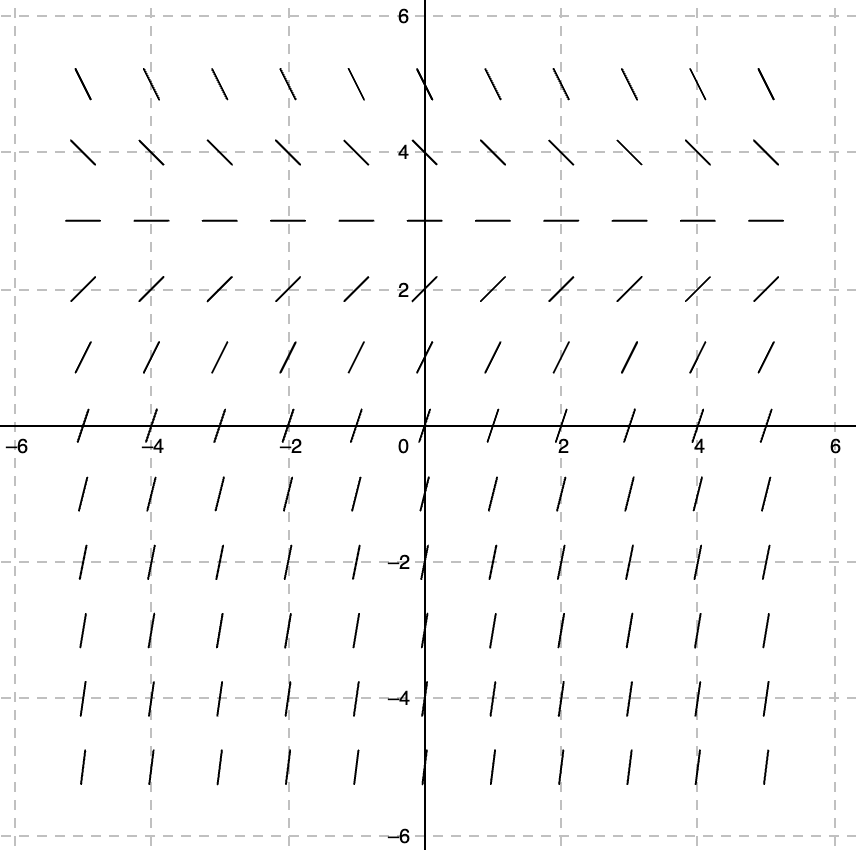
\includegraphics[scale=.5]{sf1}\end{center}
We can use this to sketch the solution to the IVP
\[\begin{cases} y' = 3-y \\
y(2)= 2 \end{cases}\]
by starting at $(2,2)$ and going along with the flow.
\begin{center}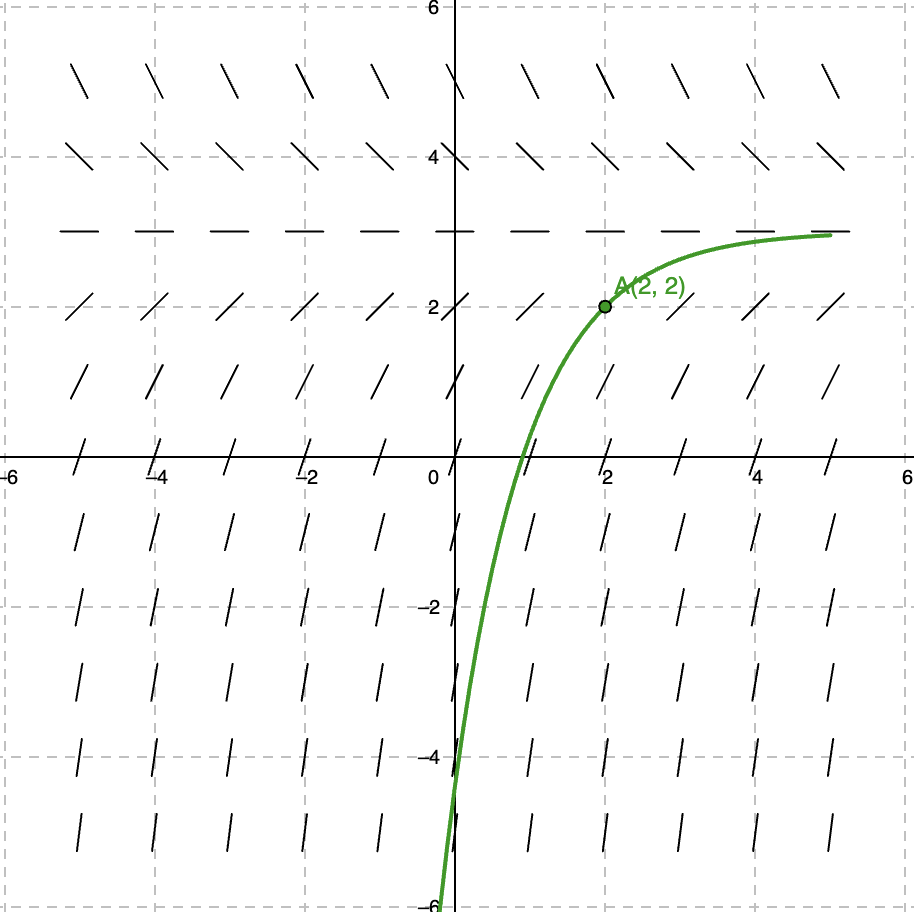
\includegraphics[scale=.5]{sf2}\end{center}

Or 
\[\begin{cases} y' = 3-y \\
y(-4)= 4 \end{cases}:\]
\begin{center}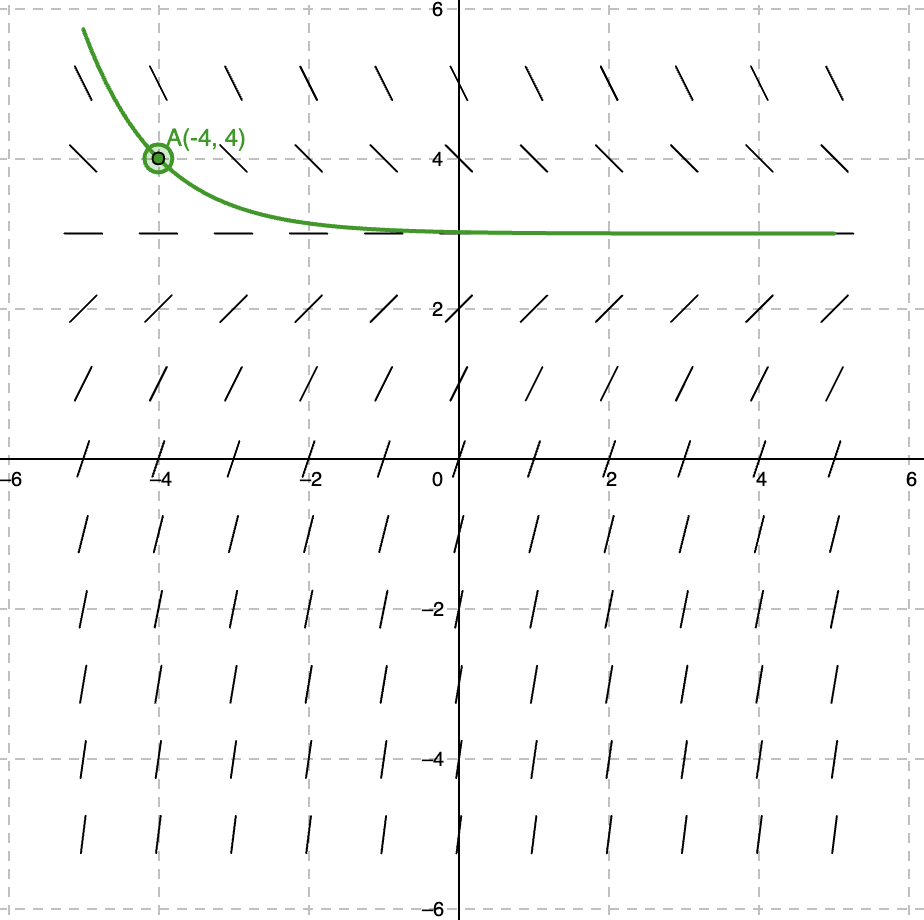
\includegraphics[scale=.5]{sf3}\end{center}
\end{ex}

The picture we drew above is called a \emph{slope field}.\index{slope field}

\subsection*{Discussion Questions} Draw a slope field for the differential equation
\[ y'= x+y\] and use it to sketch the solutions with initial conditions
\begin{enumerate}
\item $(0,1)$
\item $(0,0)$
\item $(0,-1)$
\item $(0,-2)$
\end{enumerate}
\begin{framed}
\begin{center}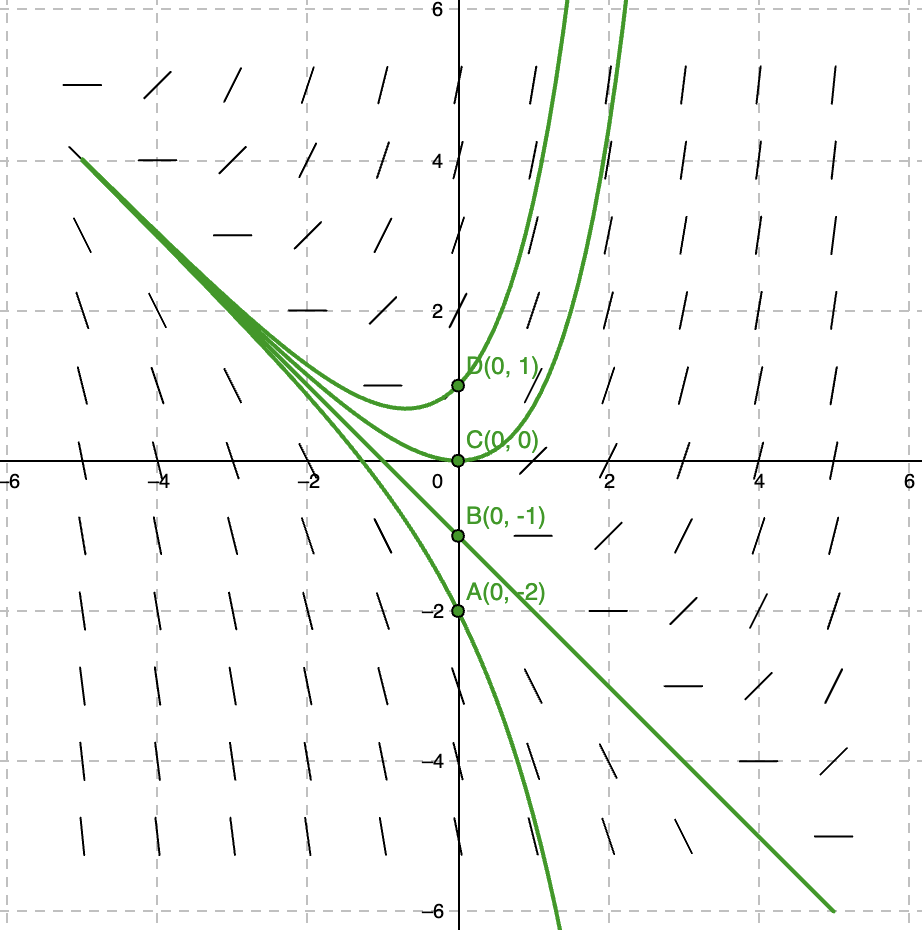
\includegraphics[scale=.5]{sf4}\end{center}
\end{framed}

%\begin{comment}



\Sept{1}

\begin{ex} As we discussed, we can use slope fields to try to understand solutions of an IVP without finding a formula for an explicit solution. Let's return to our counterfeiting example (where new good and bad bills were being introduced, and the banks replaced bad ones with good ones). We found the following IVP for our situation:
\[ \begin{cases} C'(t) = 1-\frac{2C}{10+t} \\
C(0)=10\end{cases}.\]
We wanted to know whether the number of counterfeits would continue to grow (and if so, how fast).
Let's sketch a slope field for our differential equation:
\begin{center}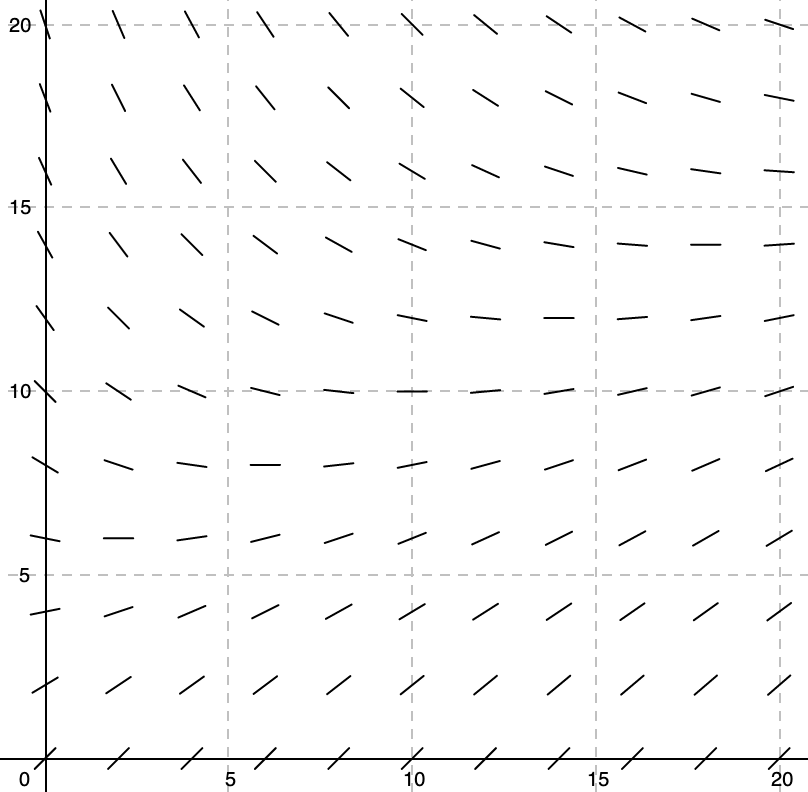
\includegraphics[scale=.5]{sf7}\end{center}
and sketch a curve for the initial condition:
\begin{center}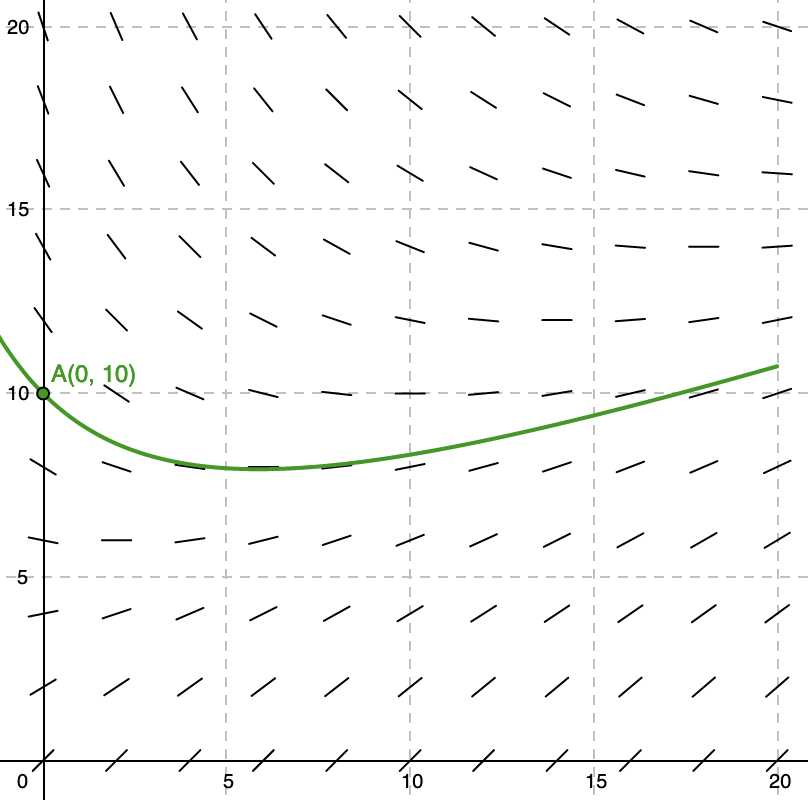
\includegraphics[scale=.5]{sf8}\end{center}
It looks like the number of counterfeits decreases at first and maybe starts to rebound. We will solve this analytically very soon to confirm our guess.
\end{ex}




\subsection*{Autonomous differential equations}
Example~\ref{ex:first aut} belongs to a class of equations that is worth singling out.
\begin{defn} A differential equation of the form \[ y' = f(y)\]
 is said to be \emph{autonomous}.\index{autonomous}
 \end{defn}
 
 The behavior of a solution of an autonomous differential equation is determined entirely by the current value of the function (and not the independent variable).
 
For an autonomous differential equation, whether a solution is increasing, decreasing, or constant at a point only depends on the $y$-value at that point. We can determine this either algebraically or using the slope field.

\begin{ex}
Consider the autonomous differential equation 
\[ y' = y^3 - 2y^2.\]
To figure out when $y$ is increasing, we figure out when $0<y' =  y^3 - 2y^2$.
We do a little algebra to figure out. Factoring, we see that the zeroes of the right-hand side are $0$ and $2$, so the sign of $y$ can only change at $0$ and $2$. On $(-\infty, 0)$, $y^3 - 2y^2<0$; at $0$, it is zero; on $(0,2)$ it is negative; at $2$, it is $0$; on $(2,\infty)$, it is positive.

Thus, a solution $y$ is increasing when $2 < y <\infty$, is decreasing on $(-\infty,0) \cup (0,\infty)$, and is constant if $y=0$ or $2$.

We can also use the slope field to determine when it is increasing or decreasing.
\begin{center}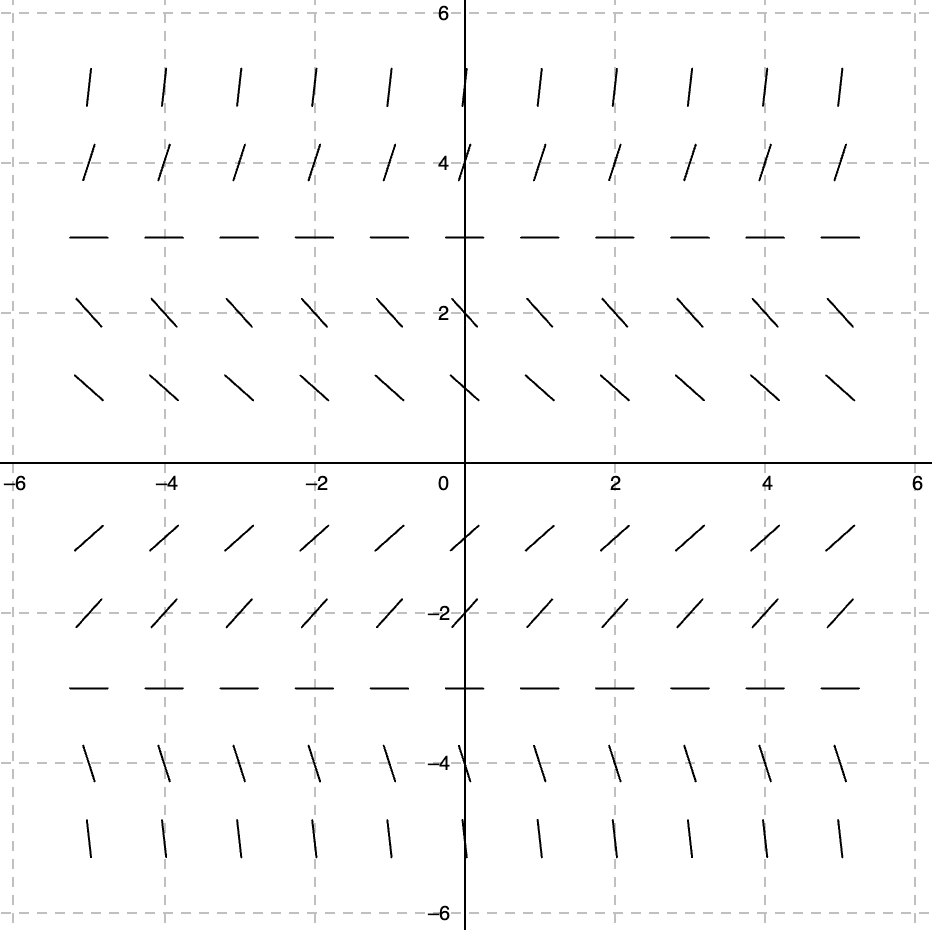
\includegraphics[scale=.5]{sf5}\end{center}
Let's sketch some solutions:
\begin{center}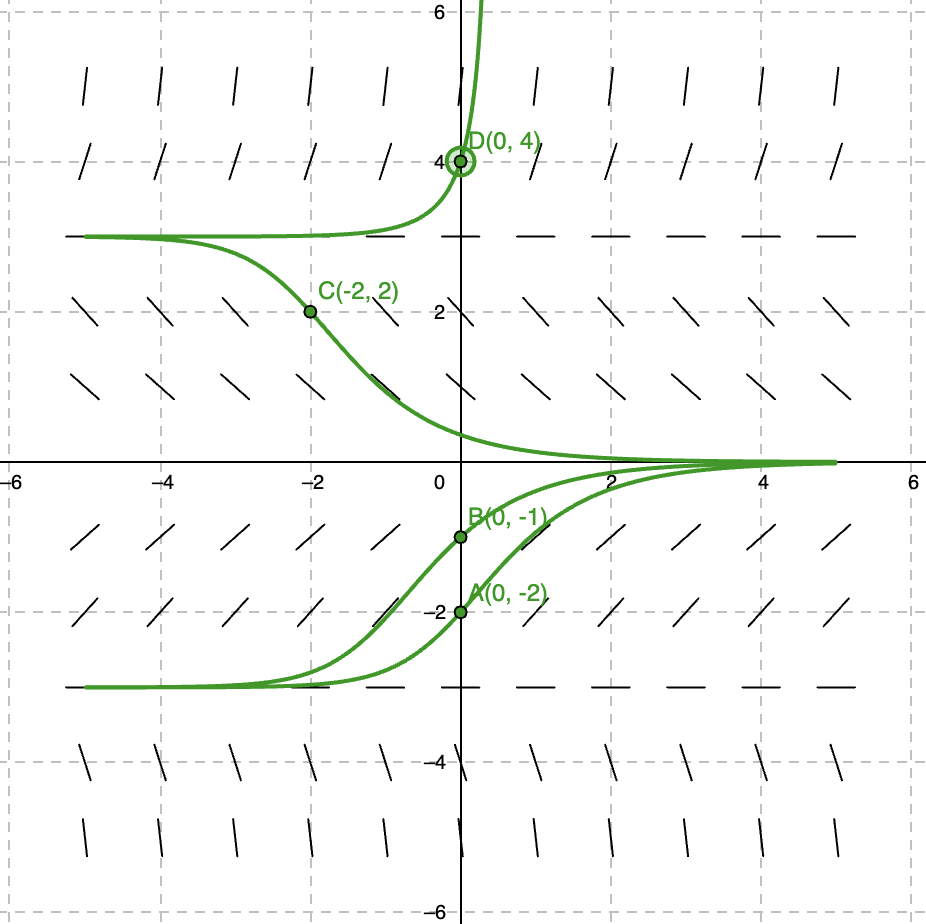
\includegraphics[scale=.5]{sf6}\end{center}
\end{ex}

A constant solution to an autonomous differential equation is also called an \emph{equilibrium solution}\index{equilibrium solution}.


\subsection*{Review of integration} Now we will start to collect some techniques for solving differential equations. Of course integration will play a big role. Let's review some basic techniques of integration. We will usually be using \emph{indefinite integration} or \emph{antidifferentiation} in this class. First, let's recall a list of building block functions whose integrals we need to know. 

\begin{itemize}
\item $\int x^n \, dx = \frac{x^{n+1}}{n+1} + C$ when $n\neq -1$.
\item $\int \frac{1}{x} \, dx = \ln|x| + C$.
\item $\int e^x \, dx = e^x + C$.
\item $\int \sin(x) \, dx = -\cos(x) + C$.
\item $\int \cos(x) \, dx = \sin(x) + C$.
\end{itemize}

Here are a couple more special ones.

\begin{itemize}
\item $\int \frac{dx}{\sqrt{1-x^2}} = \arcsin(x) + C$.
\item $\int \frac{dx}{1 + x^2} = \arctan(x) + C$.
\end{itemize}

We also have many rule for how to integrate complicated functions in terms of integrating smaller parts. There are two easy rules to get us started.

\begin{itemize}
\item $\int f(x) + g(x) \, dx = \int f(x)  \, dx + \int g(x) \, dx$.
\item $ \int c f(x) \, dx = c \int f(x)  \, dx$ for any constant $c$.
\end{itemize}

Unlike with derivatives, there is no direct rule for computing the integral of a composition or a product. Instead, we have ``$u$-substitutions''\index{u-substitution} and ``integration by parts''\index{integration by parts}. 

$u$-substitution is a technique that is likely to work when we can see some function and something like its derivative inside the function we are trying to integrate. In this case, we set the function to be $u$, we set $du= u'(x) \, dx$, and we try to rewrite our integrand as some function of $u$  times $du$ (and get rid of our starting variable entirely). $u$-substitutions also work well when instead of some function of $x$, we have a function of $x-a$ or a function of $ax$ for some constant $a$.
This is the main technique that we will want to use, other than the basic rules.

\begin{ex}
To compute $\int x^2 \cos(x^3) \, dx$, take $u=x^3$, so ${du=3x^2 \, dx}$. Then we have ${x^2 \, dx = \frac13 \, du}$, so our integral is \[\int \frac13 \cos(u)\,  du = {\frac13 \sin(u) + C}= \frac13 \sin(x^3) +C.\]
\end{ex}


Integration by parts is a technique that might work when our integrand is a product of two things, one of which we know how to integrate (i.e., looks like the derivative of something). The general rule is if we can find functions $u(x), v(x)$ such that our integral is $\int u \, dv$ (where $dv = v'(x) \, dx$), the we have
\[ \int  u \, dv = uv -  \int v \, du;\]
and if we can integrate $ \int v \, du$, we are done. A rule of thumb for what to choose for $u$ vs what to choose for $dv$ in integration by parts is LIATE (log, inverse trig, algebraic, trig, exponential): stuff on the left is usually better for $u$'s and stuff on the right is usually better for $dv$'s.

\begin{ex}
To compute $\int x e^x \, dx$, take $u=x$ and $dv= e^x \, dx$. Then $du = dx$ and $v=e^x$. Then we have \[\int x e^x \, dx = x e^x - \int e^x \, dx = x e^x - e^x +C = (x-1) e^x +C.\]
\end{ex}

Last but not least, we have a big table of integrals in the front cover of our text. 


\Sept{6}

\subsection*{Separable first-order equations (\S2.2)} Now we are ready to solve some differential equations! First we will address first-order equations of a special form: separable eqautions.

\begin{defn} A first-order ODE is \emph{separable}\index{separable} if it can be written in the form
\[ y' = f(x) g(y)\]
for some function $f$ that only involves the independent variable and some function $g$ that only involves the dependent variable.
\end{defn}

For example,
\[ y' = x^2/y, \quad y' = \frac{3 \sqrt{y^2+1}}{\cos(x)}, \quad \text{and} \ y' = 3-y \]
are all separable (with $f(x)=x^2$ and $g(y)=1/y$ in the first one), but
\[ y' = x+y \quad \text{and} \quad y'=\sin(xy) \]
are not. Note that a separable equation may or may not be linear, but is always a first order ODE.

Here's how to solve a separable ODE: Write $y'$ as $\frac{dy}{dx}$ and pretend that the $dy$ and $dx$ are separate things. Take
\[ \frac{dy}{dx} = f(x)g(y)\]
and multiply by $dx$ and divide by $dy$ on both sides to get
\[ \frac{dy}{g(y)} = f(x) \, dx.\]
(This is why we call the equation separable: the independent and dependent variables now occur on separate sides of the equation.) Now integrate both sides:
\[ \int \frac{dy}{g(y)} = \int f(x) \, dx,\]
to get an equation for $x$ and $y$ that is no longer differential!

\begin{slogan} To solve a separable equation, separate and integrate!\end{slogan}

\begin{ex} Let's start with an equation we saw in Example~\ref{ex:first aut}:
\[ y' = 3-y.\]
Write this as 
\[ \frac{dy}{dx} = 3-y\]
and rearrange to get
\[ \frac{dy}{3-y} = dx.\]
Integrate both sides. For the LHS with use the $u$-sub $u=3-y$, so $du = - dy$. The integral becomes
\[ \int  \frac{dy}{3-y} = \int \frac{-du}{u} = -\ln|u| +C = -\ln|3-y|+C = \ln\frac{1}{|3-y|} +C.\]
We then get 
\[ \ln\frac{1}{|3-y|}  = \int  \frac{dy}{3-y} =\int \,dx = x + C.\]
Note that we only need the constant of integration on one side.
Then to solve for $y$, take exponentials:
\[ e^{\ln(\frac{1}{|3-y|})} = e^{x+C},\]
\[ \frac{1}{|3-y|} = e^{x+C}.\]
Then 
\[ |3-y| ={e^{-x-C}}\]
\[ 3-y =  \pm {e^{-x-C}}\]
\[ y =  3 \pm {e^{-x-C}}\]
Since $e^{-x-C}=e^{-x} e^{-C}$ is just some other constant $C'$ times $e^{-x}$, we could also write
\[ y= 3 + C' e^{-x}.\]
\end{ex}

\begin{ex} Take
\[ \frac{dy}{dt} = t + ty^2.\]
It doesn't look separable yet, but once we factor
\[ \frac{dy}{dt} = t (1 +y^2),\]
it becomes clear that it's separable. Separate variables:
\[ \frac{dy}{1+y^2} = t \, dt,\]
integrate:
\[ \int \frac{dy}{1+y^2} = \int t \, dt,\]
\[ \arctan(y) = \frac{t^2}{2} + C,\]
and solve for $y$ by taking tangent of both sides:
\[ y=\tan(\arctan(y)) = \tan\left(  \frac{t^2}{2} + C\right).\]
This is our general solution!
\end{ex}


\subsection*{Discussion Questions}
\begin{enumerate}
\item Which of the following equations is separable?
\begin{enumerate}
\item $y' + 2y = x^3$.
\item $\cos(x) y' = \sin(y)$.
\item $y' - xy = 1+x+y$.
\end{enumerate}
\begin{framed}
(b) and (c), but not (a)
\end{framed}
\item Find the particular solution to the IVP
\[ \begin{cases} 
e^{x} \, y' = \frac{1}{y} \\
y(0) = 1\end{cases}.\]
\begin{framed}
This is separable since we rewrite as $y' = e^{-x} \frac{1}{y}$. Then
\[ y y' = e^{-x} \rsa y  \ dy = e^{-x} \ dx \rsa \int  y  \ dy = \int e^{-x} \ dx,\]
\[ \rsa \frac{y^2}{2} = -e^{-x} + C \rsa y = \sqrt{C - 2 e^{-x}},\]
and using the initial condition,
\[ 1 = y(0) = \sqrt{C - 2 e^{0}} = \sqrt{C-2} \rsa C=3,\]
so we have
\[ y = \sqrt{3 - 2 e^{-x}}.\]
\end{framed}
\end{enumerate}

Sometimes we encounter integrals that are just impossible:

\begin{comment}
\begin{ex} Take 
\[ \frac{dy}{dt} = y e^{-t^2} \, dt\]
\[\rsa\quad \frac{dy}{y} = e^{-t^2} \, dt\]
\[\rsa\quad \int \frac{dy}{y} = \int e^{-t^2} \, dt.\]
The function $e^{-t^2}$ has no elementary antiderivative: it simply is not a function for which we have a name (in the way we usually name functions). Let's just leave it as an integral.
\[\rsa\quad \ln |y| = \int e^{-t^2} \, dt\]
\[\rsa\quad |y| = e^{\left(\int e^{-t^2} \, dt\right)}\]
\[\rsa\quad y =  \pm e^{\left(\int e^{-t^2} \, dt\right)}.\]
Here we have solved for $y$ \emph{up to an integral} in $t$.\index{solved up to an integral}
\end{ex}
\end{comment}

\subsection*{Linear equations (\S2.3)} Now we solve another large class of differential equations: first order linear ODE's.\index{first order linear ODE} Let's recall that a differential equation is a first order linear ODE if we can write it in the form
\[ a_1(t) y' + a_0(t) y = f(t)\]
for some functions $a_1(t),a_0(t),f(t)$ that only involve the independent variable $t$.

We are going to learn a magic trick to solve these: this really is a rabbit-in-the-hat idea. To motivate this wacky idea, I want to consider a couple of small examples to get the idea.

\begin{ex}
Consider the differential equation
\[ t y' + y=t^2.\]
After trying a few things, we realize this isn't separable. However, the left-hand side, as written, is interesting. Notice that, by the product rule, we have
\[ (ty)' = t y' + t' y= t y' + y.\]
Thus, we have
\[ (ty)' = t^2,\]
\[\rsa \quad ty = \int (ty)' \, dt = \int t^2 \, dt = \frac{t^3}{3} + C,\]
so \[ y = \frac{t^2}{3} + \frac{C}{t}.\]

\

That was lucky! What if we had
\[ y' + \frac{3}{t} y = t\]
instead? This is still not separable. I will magically multiply by $t^3$ to get
\[ t^3 y' + 3t^2 y = t^4.\]
By reverse product rule on the left-hand side, we have
\[ (t^3 y)' = t^4.\]
Now we integrate to get
\[ t^3 y = \int t^4 \, dt = \frac{t^5}{5} +C,\]
so \[y = \frac{t^2}{5} + \frac{C}{t^3}.\]

\

This is the idea we will use: multiply our equation through by something to turn it into an equation where the left-hand side comes from the product rule! But how do we come up with the magic multiplier?
\end{ex}

%\begin{comment}
\Sept{8}
\begin{idea}
Given a linear first order ODE of the form
\[ y' + p(t) y = q(t),\]
multiply by an \emph{integrating factor}\index{integrating factor} $\mu(t)$ so the left-hand side collapses via the product rule:
\[ \begin{array}{rcccl}
 &\mu(t) y' &+& \mu(t) p(t) y &= \mu(t) q(t)\\
 ( ?(t) y)' = &?(t) y' &+& ?'(t) y & \end{array}.\]
The mystery function $?(t)$ has to be the same as our integrating factor $\mu$, and we also have to have
\[ \mu' = \mu p(t).\]
This is separable now: we solve
\[ \frac{\mu'}{\mu} = p(t)\]
by integrating
\[ \ln |\mu| = \int p(t) \, dt,\]
and isolating $\mu$
\[ \mu = \pm e^{\int p(t) \, dt}.\]
Let's take the positive one:
Set $\mu = e^{\int p(t) \, dt}$.
\end{idea}

\begin{defn} Given a linear first order ODE of the form
\[ y' + p(t) y = q(t),\]
we call the function
\[ \mu = e^{\int p(t) \, dt}\]
the \emph{integrating factor}\index{integrating factor} of the equation. For the integrating factor, we can take just one antiderivative (i.e., ignore the constant of integration), since this is just something we're using to get a solution and not a solution.
\end{defn}

\begin{slogan}
For the linear first order ODE
\[ y' + p(t) y = q(t),\]
multiply by the integrating factor
\[ \mu = e^{\int p(t) \, dt},\]
realize the left-hand side as $(\mu y)'$,
and integrate.
\end{slogan}



Then we multiply by the integrating factor, realize the left-hand side as a result of the product rule, and integrate to solve.

\begin{ex} Let's solve the ODE that arose in our model of counterfeit currency from Aug 25. We found the equation
\[C'(t) = 1-\frac{2C}{10+t}\]
which we can write as
\[ C' + \frac{2}{10+t} C = 1.\]
The integrating factor is $\mu = e^{\int \frac{2}{10+t} \, dt}$.
We should simplify this. Set $u=10+t$, so $du = dt$, then \[\int \frac{2}{10+t} \, dt = \int \frac{2}{u} \, du = 2 \ln|u| = \ln((10+t)^2) \]
so 
\[ \mu = e^ {\ln((10+t)^2)} = (10+t)^2 .\]

Now we multiply by this integrating factor:
\[ (10+t)^2 C' + (10+t)^2\frac{2}{10+t} C = (10+t)^2\]
\[ \rsa (10+t)^2 C' + 2 (10+t) C = (10+t)^2.\]
Now we recognize the left-hand side as coming from the product rule:
\[ \big((10+t)^2 C \big)' = (10+t)^2 C' + (10+t)^2\frac{2}{10+t} C,\]
so we have
\[ \big((10+t)^2 C \big)' =(10+t)^2.\]
Now we integrate:
\[ (10+t)^2 C = \int (10+t)^2 \ dt.\]
Use the sub $u=10+t$, $du=dt$ to get
\[ \int u^2 \ du = \frac{u^3}{3} + k = \frac{(10+t)^3}{3} + k.\]
We used $k$ for the constant of integration since the name $C$ is taken!
Thus,
\[ (10+t)^2 C = \frac{(10+t)^3}{3} + k\]
\[\rsa C = \frac{10+t}{3} + \frac{k}{ (10+t)^2}.\]

We also recall our initial condition $C(0)=10$ and plug it in to get
\[ 10 = C(0) =  \frac{10+0}{3} + \frac{k}{ (10+0)^2} = \frac{10}{3} + \frac{k}{100}\]
and solve to get $k = \frac{2000}{3}$.
Thus,
\[ C(t) =  \frac{10+t}{3} + \frac{2000}{3 (10+t)^2}.\]
We can now graph this in a calculator:
\begin{center}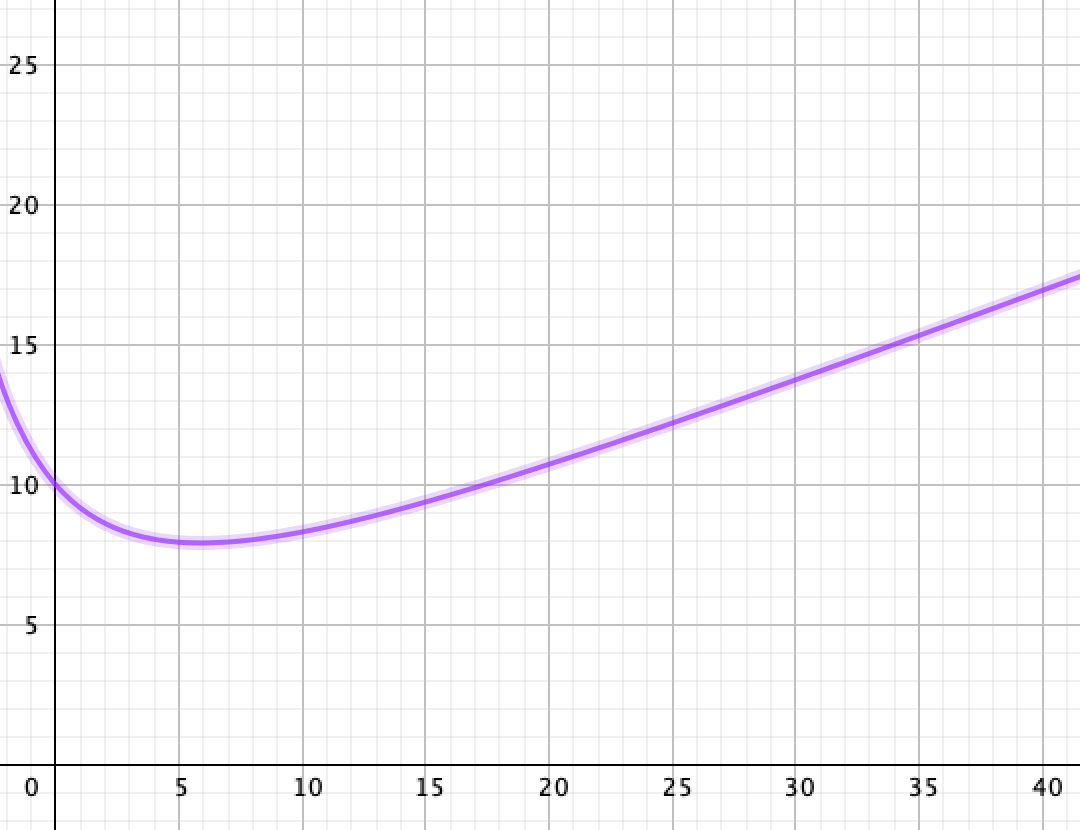
\includegraphics[scale=.5]{gr1}\end{center}
and based on the formula, we know that for $t\gg0$, the second term goes to zero, and the first term gets larger and larger. We conclude that the number of counterfeits will continue to grow in the long run!
\end{ex}

\begin{ex}
Let's solve
\[ x y' = (x+3) y = x^2 e^{-x}.\]
We need to put it in the correct form first, so divide by $x$:
\[ y' + (1+\frac{3}{x}) y = x e^{-x}.\]
In the earlier notation, $p(x) = (1+\frac{3}{x})$. The integrating factor is
\[ \mu(x)=e^{\int (1+\frac{3}{x}) \, dx} = e^{ x + 3 \ln x} = e^x  e^{\ln x^3} = e^x  x^3 = x^3 e^x.\]
Multiply by $\mu(x)$:
\[ x^3 e^x y' + (1+\frac{3}{x}) x^3 e^x = (x^3 e^x) (x e^{-x})\]
and realize LHS as coming from product rule
\[ (x^3 e^x y)' = x^4.\]
Now we integrate:
\[ x^3 e^x  y = \frac{x^5}{5} + C\]
\[ y = \frac{x^2}{5} e^{-x} + \frac{C}{x^3} e^{-x}.\]
\end{ex}

\subsection*{Discussion Questions} Find the general solution of the differential equation
\[ y' = x+ y.\]


\begin{framed}
Rearrange as $y' - y = x$. Then the integrating factor is $e^{\int -1 \, dx} = e^{-x}$. Multiply through and do the product rule backwards to get
\[ (e^{-x} y)' =e^{-x} y - e^{-x} y' = x e^{-x}.\]
We now integrate both sides. On the right, we can use integration by parts with $u=x$, $dv= e^{-x} \, dx$, $du= dx$, $v= -e^{-x}$. We get (leaving aside the constant of integration)
\begin{align*} \int x e^{-x} \, dx& = - x e^{-x} - \int (-e^{-x}) \, dx \\&= -xe^{-x} + \int e^{-x} \, dx \\&= -xe^{-x}  - e^{-x} \\&= -(x+1) e^{-x}\end{align*}
so \[ e^{-x} y = - (x+1) e^{-x} + C.\]
Then multiply through to get
\[ y = -(x+1) + C e^x.\]
\end{framed}


\Sept{13}

Let's do one more example of solving a first-order linear equation with integrating factors.

\begin{ex} Let's find the general solution to
\[ x^2 y' - y = 5.\]
First, we put it in the form from which we can read off the integrating factor:
\[ y' - \frac{1}{x^2} y = \frac{5}{x^2}.\]
Now, the integrating factor is
\[ \mu(t) = e^{\int -1/x^2 \, dx} = e^{1/x}.\]
Multiply through to get
\[ e^{1/x} y' - e^{1/x}{x^2} y = \frac{ 5 e^{1/x}}{x^2}.\]
We realize the left-hand side as $(e^{1/x} y)'$ (and we double-check it using the product rule and the chain rule):
\[ (e^{1/x} y)' = \frac{ 5 e^{1/x}}{x^2}.\]
Thus
\[ e^{1/x} y = \int \frac{ 5 e^{1/x}}{x^2} \, dx = -5 \int e^{u} \, du = -5 e^{1/x} + C.\]
using the $u$-substitution $u=e^{1/x}$, $du= -e^{1/x}/x^2 \, dx$.
Finally, we get
\[ y = -5 + C e^{-1/x}\]
as the general solution.
\end{ex}


\subsection*{Euler's Method (\S2.6)}

We now have great methods to solve certain first order ODEs, namely separable and linear ones. But this doesn't encompass all of them. There is a way to solve any IVP for first order ODE of the form
\[\begin{cases} \frac{dy}{dt} = f(t,y) \\ y(t_0) = y_0\end{cases},\]
at least approximately.  The idea is that 
\[\frac{dy}{dt}\approx \frac{\Delta y}{\Delta t} = \frac{\text{small change in $y$}}{\text{small change in $t$}},\]
which we can rewrite as \[\Delta y \cong \frac{dy}{dt} \, \Delta t.\]
So, to approximate our solution, we start at our initial value $y(t_0) = y_0$, keep adding small amounts $\Delta t$ to $t$, and each time we add
\[ \frac{dy}{dt} \, \Delta t = f(t,y) \, \Delta t \] to our $y$-value. This is the idea behind \emph{Euler's method}.\index{Euler's method}

More concretely, we fix a \emph{step size}\index{step size} $h$, which plays the role of our small change in $t$ that we called $\Delta t$. This should be a small positive number. (Though how small is a good choice can be difficult to pin down.) 

We start with the values $t_0$ and $y_0$ from the initial condition, and make a list a $t$-values $t_0,t_1,t_2,t_3,\dots$ given by the rule 
\[ t_n = t_0 + n h.\]
For the corresponding $y$-values, we go from one to the next by the rule
\[ y_{n+1}  = y_n + h f(t_n, y_n).\]

\begin{ex}
Take the IVP 
\[ \begin{cases} y' = x + y^2 \\
y(0)=0\end{cases}.\]
Let's use Euler's method with step size $1$ to approximate a solution.
We start with $x_0 = 0$ and $y_0 = 0$.
Then
\[ x_1 = 1, \quad y_1 = 0 + ( 0 + 0^2) 1 = 0\]
\[ x_2 = 2, \quad y_2 = 0 + ( 1 + 0^2) 1 = 1\dots\]
\[ x_3 = 3, \quad y_3 = 1 + ( 2 + 1^2 ) 1 = 4\]
\[ x_4 = 4, \quad y_4 = 4 + ( 3 + 4^2 )1 = 23\dots\]
Let's also try step size $h=.5$.
\[x_1 = .5 , \quad y_1 = 0+ (0+0^2) .5 = 0\]
\[x_2 = 1, \quad y_2 = 0+ \big(.5 +0^2\big) .5 = .25\]
\[x_3 = 1.5 , \quad y_3 = .25 + \big(1 +(.25)^2\big) .5 = .78125 \]
\[x_4 = 2, \quad y_4 = .78125 + \big(1.5 +(.78125)^2\big) .5 \approx 1.836425 \]

Note that the different step sizes gave different answers for $y(2)$. In general, smaller step sizes give better approximations, but take longer to compute.
\end{ex}

\subsection*{Discussion Questions}
Use Euler's method with step size $h=0.5$ to approximate a solution to 
\[\begin{cases} y' = -ty^2 \\ y(0)=1\end{cases}\]
up to $t=2$.
\begin{framed}
\[ t_0 = 0, \quad y_0=1.\]
\[ t_1 = .5, \quad y_1 = 1 + (- 0 \cdot 1^2) .5 = 1.\]
\[ t_2 = 1, \quad y_2 = 1 + (- .5 \cdot 1^2) .5 = .75\]
\[ t_3 = 1.5 , \quad y_3 = .75 + (- 1 \cdot .75^2) .5 = .46875\]
\[ t_4 = 2 , \quad y_4 = .46875 + (- 1.5 \cdot .46875^2) .5 \approx .30395\]
\end{framed}


\subsection*{Linear models (\S3.1)}

We now want to apply our ability to solve many first-order ODEs arising from real world situations, like the ones we saw in the first couple weeks.

\begin{ex} Newton's law of cooling\index{Newton's law of cooling} says that the rate at which an object cools/heats up is proportional to the difference between its temperature and the temperature of its surroundings.  First, let's state Newton's law of cooling as a general model with a differential equation.

Take $T$ to be the temperature of the heating or cooling object. We are thinking of this as changing in time, so let $t$ denote time, and think of $T$ as a function of $t$. Also, the temperature of the surroundings plays a role, so take $T_0$ to the be ambient temperature. Then the rule is
\[ \frac{dT}{dt} = k (T-T_0)\]
where $k$ is some constant of proportionality.

\Sept{15}

Let's now apply it to a specific situation. Say we place a cake in a $400^{\circ}$F oven. At first, the cake is 
 $70^{\circ}$F and after 10 minutes it is  $100^{\circ}$F. How long will it take for the cake to reach  $150^{\circ}$F?
 
Based on our story, $T_0=400$. We find the general solution of our differential equation
\[ \frac{dT}{dt} = k (T-400).\]
This is separable and linear, so we can solve it two different ways. Let's use an integrating factor.
\[T' - kT = -400 k\]
\[ \mu = e^{\int -k \, dt} = e^{-kt}\]
\[ \rsa e^{-kt} T' - k e^{-kt} T = -400k e^{-kt}\]
\[ \rsa (e^{-kt} T) ' = -400k e^{-kt}\]
\[ \rsa e^{-kt} T = \int -400k e^{-kt} \, dt = -400k \int e^{-kt} \, dt = \frac{-400k}{-k} e^{-kt} +C =400 e^{-kt} +C\]
\[ \rsa T = 400 + C e^{kt}.\]
We now have to find $C$ and $k$ for a particular function of $T$. Plug in $T(0)=70$ to get
\[ 70 = T(0) = 400 + C e^{0} = 400 + C\]
\[\rsa C= 70-400 = -330,\]
so
\[ T= 400 -330 e^{kt}.\]
Then, plug in $T(10)=75$ to get
\[ 100 = 400 - 330 e^{10 k}\]
\[\rsa -300 = -330 e^{10 k}\]
\[ \rsa \frac{10}{11} = e^{10k}\]
\[ \rsa 10k = \ln(\frac{10}{11})\]
\[ \rsa k = \ln(\frac{10}{11})/10\]
so
\[ T = 400 - 330 e^{t (\ln\frac{10}{11}) /10}.\]
Now we can set $T(t) = 150$ and solve
\[ 150 = 400 - 330 e^{t (\ln\frac{10}{11}) /10}\]
\[ \rsa -250 = -330 e^{t (\ln \frac{10}{11}) /10}\]
\[ \rsa e^{t (\ln \frac{10}{11}) /10} = 25/33\]
\[ \rsa t (\ln \frac{10}{11}) /10 = \ln(25/33)\]
\[ \rsa t = 10 \ln(\frac{25}{33}) / \ln(\frac{10}{11}) \approx 29.\]
\end{ex}

\begin{ex} We can also come up with explicit solutions for the mixing models\index{mixing model} of the type we considered earlier. Say that we have a tank of water with 300 gallons of fresh water right now. Water starts flowing out at a rate of 3 gallons per minute, and water with 5 grams of salt per gallon flows in at a rate of 6 gallons per minute. Let's find the amount of salt in the tank as a function of time.

Let $S$ be the amount of salt in the tank in grams and $t$ be time in minutes. First we note that the tank has $300 + 3t$ gallons of water after $t$ minutes. The rate of salt coming in is $5 \times 6 = 30$ grams per minute. The rate of salt going out is $3\times \frac{S}{300 + 3t} = \frac{3}{300 + 3t} S$. The differential equation modeling the situation is
\[ S' = 30 - \frac{3}{300 + 3t} S.\]
We also have the initial condition $S(0)=0$.

Our ODE is linear first-order.
\[ S' +  \frac{3}{300 + 3t} S = 30.\]
The integrating factor is
\[ \mu = e^{\int \frac{3}{300+ 3t} \, dt} = e^{\int du / u} = e^{\ln u} = u = 300+3t\]
with the $u$-sub $u=300+3t$, $du = 3 \, dt$.
\[ (300+3t) S' + 3 S = 30(300+3t)\]
\[ \rsa \big( (300+3t) S \big)' = 30(300+3t)\]
\[\rsa  (300 + 3t) S = \int 9000 + 90t \, dt = 9000 t + 45 t^2 + C\]
\[\rsa S = \frac{9000 t + 45 t^2 + C}{300 + 3t}.\]
Now we plug in the initial condition $S(0)=0$:
\[ 0 = S(0) = \frac{C}{300},\]
so $C=0$. Thus, we have
\[  S = \frac{9000 t + 45 t^2}{300 + 3t}.\]
\end{ex}

\subsection*{Logistic models (\S3.2)}

We explore an important type nonlinear first-order ODEs that commonly show up in mathematical models. One place it arises is in population growth.

\begin{ex} We discussed earlier a model of population growth wherein the rate of growth of a population of proportional to the population itself. This led to the model
\[ \frac{dP}{dt} = k P\]
where $P$ is the population considered as a function of time $t$, and $k$ is some constant of proportionality. The general solution to this is of the form
\[ P(t) = C e^{kt}.\]
This grows larger and larger and larger! A model such as this will not describe the long-term growth effectively if there is some constraint on the size of the population.

Suppose we consider a population, let's say of squirrels\index{squirrels} in the city of Lincoln. There is only so much food to go around so there should be a maximum capacity for the population; let's say that there's food enough for at most $100000$ squirrels; let's call this the \emph{total capacity}\index{total capacity}. Then $100000-P$ is the amount of room for growth in the squirrel population; let's call this the \emph{remaining capacity}\index{remaining capacity}. A \emph{logistic growth model} for the squirrel population supposes that the rate of growth of the population is \emph{jointly proportional}\index{jointly proportional} to the population $P$ and the remaining capacity $100000-P$, meaning it is proportional to the product $P (100000-P)$. That is, the logistic model says
\[ \frac{dP}{dt} = k  P (100000-P).\]
The constant $k$ we take here should be positive.
\end{ex}
%\begin{comment}
%\newpage

\Sept{20}

 \begin{ex}
Let's use our techniques from \S2.1 to analyze this equation without solving it. This is an autonomous equation, so the behavior (increasing vs decreasing vs constant) depends only on the value of $P$ and not on $t$. The right-hand side is positive when $0<P<100000$, negative when $P<0$ or $P>100000$, and constant for $P=0$ or $P=100000$. Thus, the population grows when it is positive and below capacity, decreases when above capacity, and stays constant if zero or at capacity.
\end{ex}

\begin{defn}
A \emph{logistic model}\index{logistic model} is a model that supposes that the rate of growth of some quantity $P$ is jointly proportional to $P$ and $P_c - P$ for some constant $P_c$.

A \emph{logistic equation}\index{logistic equation} is a differential equation of the form
\[ \frac{dP}{dt} = k P (P_{c} - P)\]
for some constants $k$ and $P_c$. The constant $P_c$ is called the \emph{total capacity}\index{total capacity} or \emph{carrying capacity}\index{carrying capacity}.
\end{defn}

Every logistic model can be expressed as a logistic equation.

Let's see another example.

\begin{ex} A simple model for the spread of a rumor throughout a population assumes that the rate at which the rumor spreads is jointly proportional to the number of people informed and the number of people not informed. Suppose the rumor spreads among a population of $4000$ people.
\end{ex}

\subsection*{Discussion Questions:}
\begin{enumerate}
\item Find an ODE modeling the number of people informed $I$ based the information above. (You may have an unknown constant of proportionality $k$.)
\item Based on the story, should your constant $k$ be positive or negative?
\item Based on your model (and not just the story), determine whether $I$ is increasing, decreasing, or constant, based on the number of people who know at the start.
\item Suppose that 10 people know at the start. Without solving the equation, try to sketch a graph of the solution to the IVP (even without knowing $k$!).
\end{enumerate}
\begin{framed}
We should have the equation \[ \frac{dI}{dt} = k I (4000-I).\]
Since this is presumably increasing for values of $I$ between $0$ and $4000$, then $k$ should be positive.
Now, the function $k I (4000-I)$ is zero when $I=0$ or $I=4000$, and is positive when $0<I<4000$, so we have equilibrium solutions for $I=0,4000$ and increasing solutions for $0<I<4000$.
\begin{center}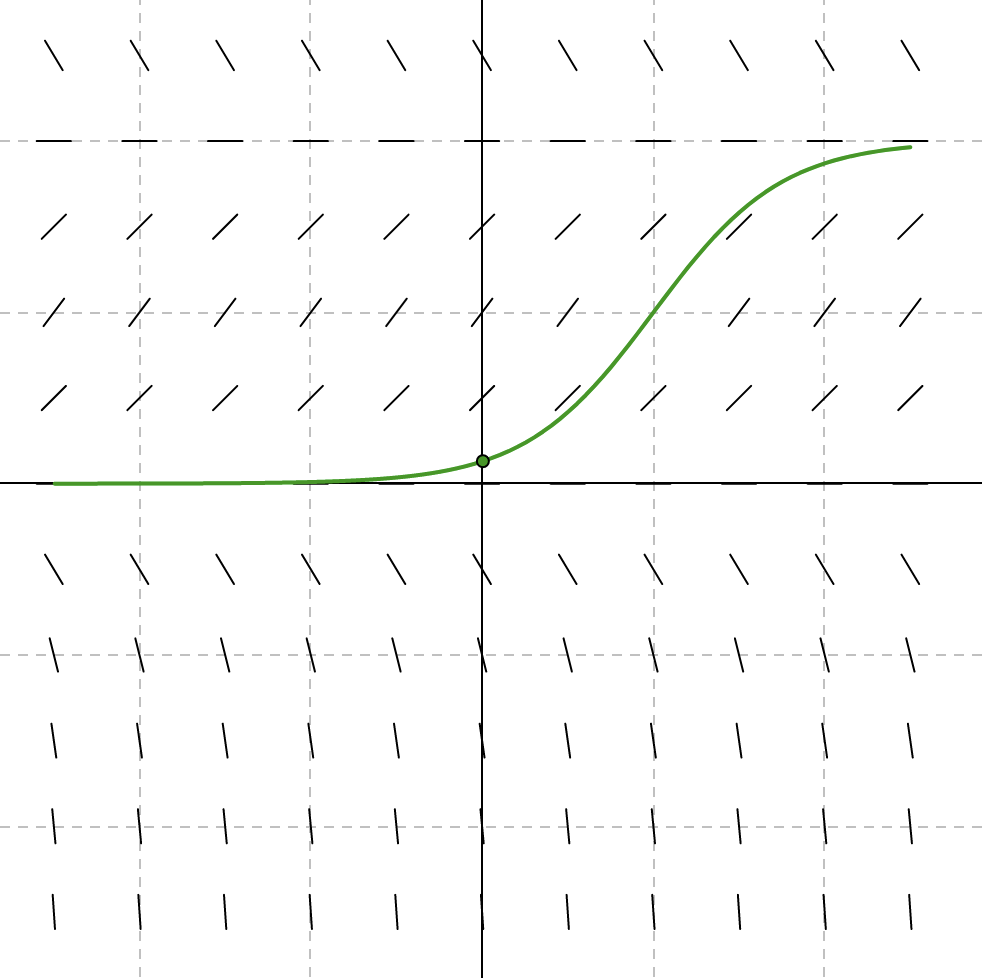
\includegraphics[scale=.5]{sf9}\end{center}
\end{framed}


The general logistic equation is separable, and we can find a general solution to it. Take
\[ \frac{dP}{dt} = k P (P_{c} - P)\]
and separate to get
\[\frac{dP}{P(P_c - P)} = k \, dt.\]
To integrate the left-hand side, we recall the trick of \emph{partial fractions}\index{partial fractions}:
we write
\[ \frac{1}{P(P_c - P)} = \frac{a}{P} + \frac{b}{P_c - P}\] for constants $a,b$ and solve:
\[ 1 = (P_c - P)a + P b = P_c a + P (b-a) \]
\[ \rsa a = 1/P_c, \ b-a = 0 ,\ b=1/P_c, \ \text{so}\]
\begin{align*} \int \frac{dP}{P(P_c - P)} &= \frac{1}{P_c} \int \frac{dP}{P} + \frac{1}{P_c} \int \frac{dP}{P_c - P} \\&= \frac{1}{P_c} \ln|P| -  \frac{1}{P_c} \ln|P_c - P| +C 
\\&= \frac{1}{P_c} (\ln|P| - \ln|P_c - P|) +C = \frac{1}{P_c} \ln \left| \frac{P}{P_c - P} \right| +C.\end{align*}
Then \[\frac{1}{P_c} \ln \left| \frac{P}{P_c - P} \right|  = kt +C\]
\[ \ln \left| \frac{P}{P_c - P} \right| = k P_c t + C\]
\[ \left| \frac{P}{P_c - P} \right| = e^{k P_c t + C} =  e^C e^{k P_c t }\]
\[ \frac{P}{P_c - P}  =   \pm e^C e^{k P_c t } \]
Since $\pm e^C$ is just a constant in any case, let's reuse the name $C$ for that other constant. Then
\[ \frac{P}{P_c - P}  = C e^{k P_c t } \]
for some new constant $C'$.
Rearranging and solving gives
\[ P = (P_c - P) C e^{k P_c t } = P_c C e^{k P_c t }  - P  C e^{k P_c t } \]
\[ \rsa P + P C e^{k P_c t }  = P_c C e^{k P_c t } \]
\[ \rsa P (1 +C e^{k P_c t } ) = P_c C e^{k P_c t } \]
\[ \rsa P = P_c \frac{C e^{k P_c t }}{1+ C e^{k P_c t }}.\]

In particular, a \emph{logistic function}\index{logistic function} can be written in the explicit form
\[ f(t) = a \frac{ b e^{ct}}{1+ b e^{ct}}\]
for some constants $a,b,c$.

In this class, you don't need to know how to solve a logistic equation or this general formula for a logistic function, just how to set one up and analyze it at we did in Sections 2.1 and 2.6.

\subsection*{Higher-order differential equations (\S4.1)}

For higher order differential equations, we will focus especially on linear equations.

\begin{defn} An ODE that can be written in the form
\[ a_n(x) y^{(n)} + a_{n-1}(x) y^{(n-1)} + \cdots + a_1(x) y' + a_0(x) y = g(x)\]
where $y^{(r)} = \frac{d^n y}{dx^r}$ is an \emph{n-th order linear equation}. If $g(x)=0$, we say that the equation is \emph{homogeneous}\index{homogeneous}; otherwise, it is \emph{nonhomogeneous}\index{nonhomogeneous}.
\end{defn}

With a first-order equation, to get a particular solution, we specified an initial condition of one value.
For a higher-order ODE, we typically need more initial conditions (or boundary conditions).

\begin{ex} Consider the differential equation
\[ y''' = 5.\]
To find the general solution, we can just integrate three times:
\[ y'' = \int 5 \, dt = 5t+ c_1\]
\[ y' = \int 5t + c_1 \, dt = \frac{5}{2} t^2 + c_1 t + c_2 \]
\[ y = \int \frac{5}{2} t^2 + c_1 t + c_2 \, dt = \frac{5}{6} t^3 + \frac{c_1}{2}  t^2 + c_2 t + c_3.\]
To get to a particular solution, we need to know more than one value of the function: we need three pieces of information of some sort to determine the three $c$'s.

One natural possibility is to specify the values at three different points. (This is an example of what we will call a \emph{boundary condition}\index{boundary condition} soon.) Another possibility is to specify the values of $y$, of $y'$, and of $y''$ at the same point. (This is what we will call an \emph{initial condition}\index{initial condition} in this setting.)

For example, given the IVP
\[ \begin{cases}
y^{(3)} = 5 \\
y(0)=1\\
y'(0)=-2\\
y''(0)=5\end{cases}\]
we solve
\[ 1 = y(0) = \frac{5}{6} \cdot 0^3 + \frac{c_1}{2}  \cdot0^2 + c_2 \cdot 0 + c_3 = c_3\]
\[ -2 = y'(0) = \frac{5}{2}\cdot  0^2 + c_1 \cdot 0 + c_2 = c_2\]
\[ 5 = y''(0) = 5 \cdot 0+ c_1 = c_1\]
so we get a unique solution
\[ y(t)= \frac{5}{6} t^3 + \frac{5}{2}  t^2 -2  t + 1.\]
\end{ex}

\begin{ex}
Suppose that we know that the solution IVP
\[ \begin{cases}
y^{(3)} + y' = 0 \\
y(\pi) = 0 \\
y'(\pi) = 2 \\
y''(\pi) = -1
\end{cases}\]

is of the form
\[ y(x) = c_1 + c_2 \sin(x) + c_3 \cos(x).\]
Let's find a particular solution using the initial conditions.
\[ 0 = y(\pi) = c_1 + c_2 \sin(\pi) + c_3 \cos(\pi) = c_1 - c_3\]
so $c_1=c_3$.
\[ 2 = y'(\pi) = c_2 \cos(\pi) - c_3 \sin(\pi) = -c_2\]
so $c_2=-2$.
\[ -1 = y''(\pi) = -c_2 \sin(\pi) - c_3 \cos(\pi) = c_3\]
so $c_3=-1$. So, our solution must be
\[ y(x) = -1 - 2 \cos(x) - \sin(x).\]
\end{ex}


\newpage

\Sept{22}

A \emph{boundary value problem}\index{boundary value problem} poses conditions at different points to get a particular solution. For example, a system of equations like
\[\begin{cases} y'' + y = 0 \\ y(a) = c \\ y(b)=d\end{cases}\] is a boundary value problem.
We will be focusing on initial value conditions, like
\[\begin{cases} y'' + y = 0 \\ y(a) = c \\ y'(a)=d\end{cases}\] 
rather than boundary value conditions in this course.

The great news is that for a linear ODE, there exist unique solutions to IVPs in the same sense we discussed for first-order equations with the Picard-Lindel\"of Theorem.

\begin{thm}[Existence and uniqueness theorem for linear IVPs]\index{existence}\index{uniqueness}
Given a linear ODE
\[ a_n(x) y^{(n)} + a_{n-1}(x) y^{(n-1)} + \cdots + a_1(x) y' + a_0(x) y = g(x)\]
where $g(x), a_0(x), \dots, a_n(x)$ are continuous and $a_n(x)\neq 0$ for all $x$, then there exists a unique solution
\[ \begin{cases} 
a_n(x) y^{(n)} + a_{n-1}(x) y^{(n-1)} + \cdots + a_1(x) y' + a_0(x) y = g(x) \\
y(t_0) = y_0\\
y'(t_0) = y_1 \\
 \quad  \vdots\\
y^{(n-1)}(t_0) = y_{n-1}
\end{cases}\]
on some interval containing $t_0$.
\end{thm}

\begin{ex} Consider the ODE
\[ (x-7) y'' + 3y = x^2 \cos(x).\]
Since $x-7=0$ when $x=7$, the theorem doesn't apply yet, so we should divide through by $x-7$:
\[ y'' + \frac{3}{x-7} y = \frac{x^2 \cos(x) }{x-7}.\]
The Theorem then says that when $\frac{3}{x-7}$ and $\frac{x^2 \cos(x) }{x-7}$ are continuous, there is a unique solution near that $x$-value: this is OK as long as $x\neq 7$.
For example, with the initial condition
\[ \begin{cases} y(-1) = 3 \\ y'(-1) = -.7\end{cases} \]
starting from $x=-1$, we know that there exists a unique solution near $x=-1$. Moreover, we can go to the left forever and to the right up until $x=7$ without getting into trouble, so this IVP has a unique solution on $(-\infty , 7)$.
\end{ex}

\subsection*{Principle of superposition}

\begin{ex}\label{ex:homog1} Consider the linear homogeneous ODE
\[ 3y'' + 2ty' + t^7 y = 0.\]
Suppose we have two solutions $y_1(t), y_2(t)$. Then for any constants $c_1,c_2$, the function
\[ y(t) = c_1 y_1(t) + c_2 y_2(t)\] is also a solution. (For example, things like $-y_1, 47 y_2, 3 y_1 - 5 y_2$ are solutions.)
Let's check it:
\begin{align*} 3 y'' + 2t y' + t^7 y &= 3 (c_1 y_1 + c_2 y_2)'' + 2t (c_1 y_1 + c_2 y_2)' + t^7 (c_1 y_1 + c_2 y_2) \\ &=3 (c_1 y_1'' + c_2 y_2'') + 2t (c_1 y_1' + c_2 y_2') + t^7 (c_1 y_1 + c_2 y_2)\\
&= c_1 (3y''_1 + 2ty'_1 + t^7 y_1) + c_2 (3y''_2 + 2ty'_2 + t^7 y_2) \\
&= c_1 (  \qquad \quad \  0 \qquad \quad \  )  \,+ \,c_2 (  \qquad \quad \  0 \qquad \quad \  ) = 0,
\end{align*}
where the last equality is because $y_1$ and $y_2$ are solutions; this means that $y$ is a solution!
\end{ex}


For about the same reason, this works for any linear homogeneous ODE: the key points were that we could ``pull out the sum and constants'' form the differential equation, which is a consequence of having a linear equation, and that a sum of constants times zero is zero, which is why we needed a homogeneous equation.  Namely, we have:

\index{Principle of superposition}
\begin{thm}[Principle of superposition for homogeneous ODEs] For any linear homogeneous ODE
\[ a_n(x) y^{(n)} +  \cdots + a_1(x) y' +  a_0(x) y = 0,\]
 given any solutions $y_1,y_2,\dots,y_t$, and any constants $c_1,c_2, \dots,c_t$, the function $y=c_1 y_1 + \cdots + c_t y_t$ is also a solution to the same equation.
\end{thm}

This is only true for linear homogeneous equations, so be sure to only apply it in that setting. We give the recipe that appears above a name.

\begin{defn} If $y_1,y_2,\dots,y_n$ are functions, we say that a function of the form $y=c_1 y_1 + \cdots + c_t y_t$ for some constants $c_1,c_2, \dots,c_t$ is a \emph{linear combination}\index{linear combination} or \emph{superposition}\index{superposition} of the functions $y_1,y_2,\dots,y_t$.\end{defn}

Let's return to our example and see what happens if the equation is nonhomogeneous instead.
\begin{ex} Consider the linear nonhomogeneous ODE
\[ 3y'' + 2ty' + t^7 y = \sin(t).\]
%and
%\[ 3y'' + 2ty' + t^7 y = \cos(x).\]
%They are linear and have the same left-hand side ($y$ and its derivatives part), but different right-hand sides (doesn't depend on $y$ part).
Suppose we have a solution $y_1(t)$ to this equation and we want to get another one. Based on the homogeneous case, we might the try something like $y=c_1 y_1 + c_2 y_2$ for some constants $c_1,c_2$ and some other function $y_2$. What changes? In the last line of computation of Example~\ref{ex:homog1}, the first and last zeroes should now be $\sin(x)$. The $c_1$ is going to mess things up, so we better hold off of it; the rest is OK as long as we still the second $0$. This means we are OK to take $y= y_1 + c_2 y_2$ for a solution $y_2$ of the homogeneous equation with the same ``left-hand side''!
\end{ex}

Again, for about the same reason, this works for any linear ODE.  Namely, we have:

\index{Principle of superposition}
\begin{thm}[Principle of superposition for nonhomogeneous ODEs] 
For any linear nonhomogeneous ODE
\[ a_n(x) y^{(n)} +  \cdots + a_1(x) y' +  a_0(x) y = g(x),\]
given one particular solution $y_p$, and some solutions $y_1, \dots,y_t$ of the corresponding homogeneous equation
\[ a_n(x) y^{(n)} +  \cdots + a_1(x) y' +  a_0(x) y = 0,\]
and any constants $c_1,c_2, \dots,c_t$, the function
$y = y_p + c_1 y_1 + \cdots + c_t y_t$ is also a solution to the first equation.
\end{thm}



\subsection*{Discussion Questions}
The functions $e^x$ and $e^{2x}$ are solutions to
\[ y'' - 3y' + 2y = 0,\]
and  $-xe^{x}$ is a solution to
\[ y'' - 3y' + 2y = e^{x}.\]
Consider the following functions:
\begin{multicols}{2}
\begin{enumerate}[label=(\alph*)]
\item\label{10a} $y= 5 e^x$
\item\label{10b} $y= e^x - e^{2x}$
\item\label{10c} $y= 7 xe^{x}$
\item\label{10d} $y= 12e^x -  3 e^{2x}$
\item\label{10e} $y=  -2 e^x - xe^{x}$
\item\label{10f} $y= -2 x e^x + 3 e^{2x}$
\item\label{10g} $y= - x e^x + 9 e^{2x}$
\item\label{10h} $y= 4 e^{2x} - x e^x + 15 e^{2x}$
\end{enumerate}
\end{multicols}
According to the superposition principle determine:
\begin{enumerate}
\item Which of the functions are solutions to
\[ y'' - 3y' + 2y = 0\ ?\]
\item Which of the functions are solutions to
\[ y'' - 3y' + 2y = e^x\ ?\]
\end{enumerate}
\begin{framed}
\begin{enumerate}
\item Since this is a linear homogeneous equation, we know that any superpositions of our given solutions $e^x$ and $e^{2x}$ are also solutions of the equation. This means \ref{10a}, \ref{10b}, and \ref{10d} are solutions too.
\item Since this is a linear nonhomogeneous equation, we know that our particular solution plus any superposition of our homogeneous solutions is also a solution. This means \ref{10e}, \ref{10g}, and \ref{10h} are solutions too.

The other functions \ref{10c} and \ref{10f} are not solutions to either!
\end{enumerate}
\end{framed}


\Oct{4}


	\subsection*{Discussion Questions}
	
	
	Consider the differential equations
	\begin{equation}\tag{$\clubsuit$} y'' + \sin(t) y' + e^{t^2} y = 0 \end{equation}
		\begin{equation}\tag{$\diamondsuit$} y'' + \sin(t) y' + e^{x^2} y = \tan(t) \end{equation}
	
	\
	
\begin{enumerate}
\item What is the order of these equations? Are they linear? Are the homogeneous?

\begin{framed}
Second order, linear, first is homogeneous, second is not.
\end{framed}

\item Say that we have solutions $f(t)$ and $g(t)$  to equation $(\clubsuit)$, and a solution $h(y)$  to equation $(\diamondsuit)$. 
Which of the following definitely are solutions to $(\clubsuit)$? Which definitely are solutions to $(\diamondsuit)$? 
\begin{multicols}{3}
\begin{enumerate}
\item\label{11a} $y= 2f$
\item\label{11b} $y= 2h$
\item\label{11c} $y=3f-g$
\item\label{11d} $y=f^2$
\item\label{11e} $y=0$
\item\label{11f} $y=g+h$
\item\label{11g} $y=tg$
\item\label{11h} $y=h-4f$
\end{enumerate}
\end{multicols}
\begin{framed}
\noindent \ref{11a}, \ref{11c}, \ref{11e} are solutions to $(\clubsuit)$ and \ref{11f}, \ref{11h} are solutions to~$(\diamondsuit)$.
\end{framed}


\item What can you say about existence and uniqueness of the following initial value problems? Are they true on some interval? If so, what's the biggest such interval?
\begin{enumerate}
\item \[ \begin{cases} y'' + \sin(t) y' + e^{t^2} y = 0 \\ 
y(0.2) = 4 \\
y'(0.2) = \pi
\end{cases}\]
\begin{framed}
Exists and unique on $(-\infty,\infty)$.
\end{framed}
\item \[ \begin{cases} y'' + \sin(t) y' + e^{t^2} y = \tan(t) \\ 
y(0.2) = 4 \\
y'(-0.1) = \pi
\end{cases}\]
\begin{framed}
Exists and unique on $(-\pi/2,\pi/2)$.
\end{framed}
\item \[ \begin{cases} y'' + \sin(t) y' + e^{t^2} y = 0 \\ 
y(0.3) = 7 \\
\end{cases}\]
\begin{framed}
Exists but not unique on  $(-\infty,\infty)$.
\end{framed}
\end{enumerate}
\end{enumerate}

We are going to put the principle of superposition to use to write general solutions of linear ODEs in terms of a few solutions. Namely, for a homogeneous linear ODE, we will express the general solution as
\[ y = C_1 y_1 + \cdots + C_t y_t\]
for functions $y_1,\dots,y_t$ (that we have to go find in each case).
For a nonhomogeneous linear ODE, we will express the general solution as
\[ y = y_p + C_1 y_1 + \cdots + C_t y_t\]
where $y_p$ is any \emph{particular solution}\index{particular solution} and $C_1 y_1 + \cdots + C_t y_t$ is the general solution to the associated homogeneous ODE.

We would like a way to figure out when we have found enough solutions $y_i$ to make all of them by superposition. Before we can do it, we need a way to say that an extra solution is new.

%For example, the general solution of $y'' - 3y' + 2y = 0$
%is \[y= C_1 e^{x} + C_2 e^{2x}\]
%and the general solution of  $y'' - 3y' + 2y = e^{x}$
%is \[y= -x e^x + C_1 e^{x} + C_2 e^{2x}:\] here $-x e^x$ is a particular solution and $C_1 e^{x} + C_2 e^{2x}$ is the complementary solution.

\subsection*{Linear dependence and Wronskians}

\begin{ex} Consider the ODE
\[ y'' - y=0\]
(equivalently, $y'' = y$).
Certainly $y_1= e^x$ is a solution, since its derivative is itself.
Can we guess another? $y_2= e^{-x}$ has its negative for its derivative, and then the sign flips again with the second derivative, so this is also a solution.

By the principle of superposition, $7 e^x$ and $-15 e^x + \pi e^{-x}$ are also solutions. Note that something like $x e^x$ is not a solution: the principle only applies to constant multipliers.

Let's recall a couple more functions:\index{$\sinh(x)$}\index{$\cosh(x)$}
\[ \sinh(x) = \frac{e^x - e^{-x}}{2} \quad \cosh(x) = \frac{e^x + e^{-x}}{2}\]
are functions that satisfy $\sinh'(x) = \cosh(x)$ and $\cosh'(x) = \sinh(x)$,
so $y_3=\sinh(x)$ and $y_4=\cosh(x)$ are also solutions.

However, $y_3 = \frac12 y_1 - \frac12 y_2$ and $y_4 = \frac 12 y_1 + \frac12 y_2$ are already explained by $y_1$ and $y_2$ using the principle of superposition, so we don't really need $y_3$ or $y_4$ to create the other solutions. That is, using linear combinations, $\{y_1,y_2\}$ can be used to build everything that $\{y_1,y_2,y_3,y_4\}$ can. Note that we can also build everything using $\{y_3,y_4\}$.

The upshot is that $\{y_1,y_2,y_3,y_4\}$ has redundancy for forming linear combinations.
\end{ex}

We want a tool for detecting redundancy like this.

In the last example, the equation
\[ \frac12 y_1 + \frac12 y_2 = y_4\]
can be rewritten as
\[ \frac12 y_1 + \frac12 y_2 + 0 y_3 + (-1) y_4   = 0.\]

\begin{defn} We say that a set of functions $\{y_1,\dots, y_n\}$ is \emph{linearly independent}\index{linearly independent} (i.e., no redundancy) if whenever some linear combination yields the zero function
\[ c_1 y_1 + \cdots + c_n y_n = 0\]
the coefficients $c_1,\dots,c_n$ must be $0$. Otherwise $\{y_1,\dots, y_n\}$ is \emph{linearly dependent}\index{linearly dependent}.
\end{defn}

For example, 
\[ \frac12 e^x + \frac12 e^{-x} + (-1) \cosh(x) = 0\]
means that $\{e^x,e^{-x}, \cosh(x)\}$ is linearly dependent.


We now want a tool to detect linear (in)dependence of functions. Here is Wronski's clever idea: if $c_1 f + c_2 g=0$ (as functions) then, taking derivatives,
 \[ c_1 f' + c_2 g' = 0\] also. Then \[f g' - f' g = f (\frac{-c_1}{c_2} g') - f' (\frac{-c_1}{c_2} g) =0.\]
 
 \begin{defn} The \emph{determinant}\index{determinant} of a $2\times 2$ matrix
 \[ \begin{bmatrix} a & b \\ c& d\end{bmatrix}\]
 is
  \[ \det \begin{bmatrix} a & b \\ c& d\end{bmatrix} = ad-bc.\]
  The \emph{determinant}\index{determinant} of a $3\times 3$ matrix
 \[ \begin{bmatrix} a & b & c\\ d & e & f \\ g & h & i \end{bmatrix}\]
 is
\[\det \begin{bmatrix} a & b& c\\ d & e & f \\ g & h & i \end{bmatrix} = \raisebox{-6.7mm}{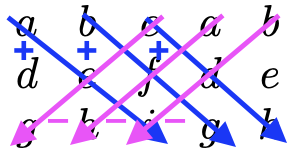
\includegraphics[scale=.55]{det1}} = aei+bfg+cdh - ceg - afh-bdi.\]
\end{defn}

Larger square matrices have determinants too, but we won't discuss them in this class. Do not attempt to generalize the formula for $3\times 3$ to $n\times n$ matrices; consult a linear algebra text instead.


\Oct{6}

\begin{defn} The \emph{Wronskian}\index{Wronskian} of two functions $f,g$ is the determinant
\[ W(f,g) = \det \begin{bmatrix} f & g \\ f'  & g' \end{bmatrix} = f g' - f' g.\] This is a function (of the same variable that $f$ and $g$ are functions of).
The  \emph{Wronskian} of three functions $f,g,h$ is the determinant
\[ W(f,g,h) = \det \begin{bmatrix} f & g & h  \\ f' & g' & h' \\ f'' & g'' & h''\end{bmatrix}.\]
In general, the Wronskian of $n$ functions is the determinant of an $n\times n$ matrix involving the first $n-1$ derivatives of the functions.
\end{defn}

For example, \[W(x^2,x^3) = \det \begin{bmatrix} x^2 & x^3 \\ 2x & 3x^2 \end{bmatrix} = x^2 \cdot 3x^2 - 2x \cdot x^3 = x^4.\]

The point of Wronskians is the following:
\begin{thm} A set of function $\{f_1,\dots,f_n\}$ (with at least $n-1$ derivatives) is linearly dependent on an interval if and only if the Wronskian $W(f_1,\dots,f_n)$ is the  zero function on that interval.
\end{thm}

\begin{ex}
Let's use Wronskians to show that the functions $\{ x, e^x\}$ are linearly independent on $(-\infty,\infty)$. We have
\[ W( x, e^x) = \det \begin{bmatrix} x & e^x \\ 1 & e^x\end{bmatrix} = xe^x - e^x = (x-1) e^x\] which is not the zero function, so the are linearly independent.

Let's try $\{1,  x^2, 4-x^2\}$ instead on $(-\infty,\infty)$. We have
\[\begin{aligned} W(1,  x^2, 4-x^2) &= \det \begin{bmatrix} 1 & x^2 & 4-x^2 \\ 0 & 2x & -2x \\ 0 & 2 & -2 \end{bmatrix} \\& = 1 \cdot 2x \cdot (-2) + x^2 \cdot (-2x) \cdot 0 + (4-x^2) \cdot 0 \cdot 2 \\&\quad - (4-x^2) \cdot 2x \cdot 0 - 1 \cdot (-2x) \cdot 2  - x^2 \cdot 0 \cdot -2 = 0,\end{aligned}\]
so these are linearly dependent.
\end{ex}

In fact, when we have a set of solutions to a homogeneous linear ODE, something even better happens.

\begin{fact}
If $f_1,\dots,f_n$ are $n$ solutions of an $n$th order homogenous linear equation on some interval, then 
\begin{enumerate}
\item $f_1,\dots,f_n$ are linearly dependent on the interval $\Longleftrightarrow$ if the Wronskian function $W(f_1,\dots,f_n)$ is \emph{always} equal to zero on the interval.
\item $f_1,\dots,f_n$ are linearly independent on the interval $\Longleftrightarrow$ the Wronskian function $W(f_1,\dots,f_n)$ is \emph{never} equal to zero on the interval.
\end{enumerate}
\end{fact}

This means that we can check the Wronskian function at any single point (of your choice!), and whether it's zero or not determines whether the solutions are independent or not.


Now we come to our key definition.

\begin{defn} For an $n$th order homogeneous linear ODE, a \emph{fundamental set}\index{fundamental set} of solutions is a collection of $n$ (same number!) linearly independent solutions.
\end{defn}

\begin{thm}[General solutions for linear ODEs] \quad
\begin{enumerate} 
\item
Given an $n$th order homogeneous linear ODE,
\[ a_n(x) y^{(n)} + a_{n-1}(x) y^{(n-1)} + \cdots + a_1(x) y' + a_0(x) y = 0\]
there is a fundamental set of solutions $y_1,\dots,y_n$. Given such a fundamental set, the general solution of the ODE is
\[y = C_1 y_1 + \cdots + C_n y_n.\]
\item Given an $n$th order nonhomogeneous linear ODE,
 \[ a_n(x) y^{(n)} + a_{n-1}(x) y^{(n-1)} + \cdots + a_1(x) y' + a_0(x) y = g(x),\]
 and any particular solution $y_p$, the general solution is 
\[y = y_p + C_1 y_1 + \cdots + C_n y_n,\]
where $\{y_1,\dots,y_n\}$ is a fundamental set of solutions to the associated homogeneous equation.
\end{enumerate}
\end{thm}

\begin{slogan} Given $n$ solutions to an $n$-th order homogeneous linear ODE, if their Wronskian is nonzero, then they form a fundamental set, and the general solution is given by superposition. \end{slogan}



\begin{ex}
Consider the ODE
\[ y'' - 3y' + 2y = 0.\]
We saw that $y=e^x$ and $y=e^{2x}$ are two solutions to this equation. We want to use these to express the general solution. If we have two linearly independent solutions, the general solution is given by superposition. We check the Wronskian:
\[ W(e^x,e^{2x}) = \det \begin{bmatrix} e^x & e^{2x} \\ e^x & 2 e^{2x} \end{bmatrix} = e^x (2e^{2x}) - e^x e^{2x} = e^{3x} \neq 0,\]
so they are linearly independent. Thus the general solution is
\[ y = C_1 e^x + C_2 e^{2x}.\]

Now we consider 
\[y'' - 3y' + 2y = e^{x}.\]
We saw earlier that $y=-xe^x$ is a solution. Using what we just proved about the homogeneous solution, we conclude that
\[ y=-xe^x + C_1 e^x + C_2 e^{2x}\]
is the general solution to this nonhomogeneous equation.
\end{ex}

\subsection*{Discussion Questions}
\begin{enumerate}
\item
We saw that $e^x$ and $e^{-x}$ are solutions of $y'' = y$.
Is $\{e^x,e^{-x}\}$ a fundamental set? 
\item Check that $e^{x-1}$ is also a solution to $y'' = y$.
Is $\{e^x,e^{x-1}\}$ a fundamental set? 
\item What is the general solution to $y'' = y$?
\item We also saw that $\sinh(x),\cosh(x)$ are solutions.
Is $\{\sinh(x),\cosh(x)\}$ a fundamental set? 
\end{enumerate}
\begin{framed}
\begin{enumerate}
\item
Yes: $W(e^x,e^{-x}) = -2 \neq 0$.
\item No: $W(e^x,e^{x-1}) = 0$.
\item $y = C_1 e^x + C_2 e^{-x}$.
\item Yes: We can use the fact and check the Wronskian just at $x=0$: Using my calculator,
$\sinh^2(0) - \cosh^2(0) = -1$.
\end{enumerate}
Note that we can write the general solution either as 
\[ C_1 e^x + C_2 e^{-x}\]
or as 
\[ C_1 \sinh(x) + C_2 \cosh(x)\]
and both are right: the collection of functions we can make by either recipe is the same!
\end{framed}


\subsection*{Reduction of order (\S4.2)}\index{reduction of order}

We know that for a homogeneous linear ODE of order two, we are looking for two linearly independent solutions to form a fundamental set. Before we start to discuss methods to find solutions, we are going to discuss a method to get a second solution if we already know one. 

Here is the idea:  Given \[ a_2(x) y'' + a_1(x) y' + a_0(x) = 0\] and one solution $y_1(x)$, we are going to look for a function that is a nonconstant multiple of $y_1(x)$:  $y_2(x) = u(x) y_1(x)$. When we plug it in, we can turn it into a first order ODE, which we already know how to solve.

%\begin{ex} Consider the ODE
%\[ y'' + y' - 2y = 0.\]
%I found $y_1 = e^x$ is a solution:
%\[ (e^x)'' + (e^x)' - 2 e^x = e^x + e^x - 2 e^x = 0.\]
%Let us use reduction of order to find another one. We take $y_2= u e^x$ and plug it in:
%\[ (u e^x)'' + (u e^x)' - 2 (u e^x) = 0\]
%\[ (u' e^x + u e^x) ' + (u' e^x + u e^x)- 2 (u e^x) = 0\]
%\[ (u'' e^x + u' e^x + u' e^x + u e^x) + (u' e^x + u e^x)- 2 (u e^x) = 0\]
%We want to think of this as an equation in $u$, so group by the derivatives of $u$.
%\[ u'' e^x + u' (3 e^x) + u (2 e^x - 2 e^x) = 0\]
%\[ u'' e^x + 3 u' e^x= 0\]
%This looks like a second order equation, but take $v= u'$. We now have
%\[ v' e^x + 3 v e^x = 0.\]
%\[ v'  + 3 v  = 0.\]
%\[ v'  = -3 v.\]
%We know a solution of this is $v=Ce^{-3x}$. Then $u= \frac{-1}{3} C e^{-3x} + C'$. We only want one solution $u$, so $e^{-3x}$ works. Now take $y_2 = e^x e^{-3x} = e^{-2x}$.
% We can check:
% \[ (e^{-2x})'' + (e^{-2x})' - 2 e^{-2x} = 4 (e^{-2x})  - 2 (e^{-2x}) - 2 e^{-2x} = 0.\]
% Finally, let's hcek that our two solutions are linearly independent with the Wronskian:
% \[ W(e^{x},e^{-2x}) = \det \begin{bmatrix} e^x & e^{-2x} \\ e^{x} & -2 e^{-2x} \end{bmatrix} = -2 e^x e^{-2x} - e^x e^{-2x} = -3 e^{-x} \neq 0.\]
% We conclude that the general solution is 
% \[ C_1 e^x + C_2 e^{-2x}.\]
% \end{ex}

\begin{ex} Consider the second-order ODE
\[ y'' - \frac{1}{t} y' + \frac{1}{t^2} y = 0.\]
Out of nowhere, consider $y_1= t$.
We have $y_1 ' = 1$, and $y'' = 0$, so
\[ 0 - \frac{1}{t} 1 + \frac{1}{t^2} t = 0\]
and this is a solution.
Let's use ``reduction of order'' to find another solution. We know that we just need one more linearly independent solution! We plug in $y_2= u y_1 = u t$, where $u$ is an unknown function of $t$ to be determined, as a guess.
Plug in this $y_2$ to the equation:
\[ (u t)'' -  \frac{1}{t} (ut)' + \frac{1}{t^2} (ut) = 0.\]
\[ (ut)' = u' t + u \qquad (ut)'' = (u' t + u )' = u'' t + u' + u' = u'' t + 2 u'.\]
\[ \rsa (u'' t + 2 u') -  \frac{1}{t} (u' t + u) + \frac{1}{t^2} (ut) = 0.\]
We are thinking of $u$ as our variable, so we want to bring together the different derivatives of $u$:
\[ \rsa t u''  + u' =0 .\]
This is second order in $u$ (darn!) but is first order in $u'$! To see it, set $v=u'$ (so $v'=u''$):
\[ t v' + v = 0.\]
\[ v' + \frac{1}{t} v = 0.\]
We know how to solve this!
Take the integrating factor $\mu = e^{\int \frac{1}{t} \, dt} = e^{\ln t} = t$, so
\[ (tv)' = tv' + v = 0\]
\[\rsa tv = C \quad \rsa v= C/t. \]
Then remember $v=u'$, so
\[ u' = C/t \quad \rsa u= C \ln t + C'.\]
And finally
\[ y_2 =  (C \ln(t) + C')t = C t \ln t + C' t\]
but since we are only looking for one solution, let's just go with the interesting part ($C=1, C'=0$):
\[ y_2 = t \ln(t).\]

Let's check that $y_1$ and $y_2$ are linearly independent:
\begin{align*} W( t, t \ln(t) ) &=  \det \begin{bmatrix} t & t \ln(t) \\ (t)' &(t \ln(t))' \end{bmatrix} \\&= \det \begin{bmatrix} t & t \ln(t) \\ 1 & \ln(t) + 1 \end{bmatrix} = t(\ln(t) +1) - t(\ln(t)) = t\neq 0,\end{align*}
so they are!

We conclude that $t$ and $t \ln(t)$ form a fundamental set of solutions; i.e., the general solution of the equation is
\[ y =C_1 t + C_2 t \ln(t).\]
\end{ex}
 

 

\begin{slogan}
Given a solution $y_1$ of a second-order homogeneous linear ODE, plug in $y_2= u y_1$, and get a first-order homogeneous linear ODE in terms of $v=u'$. Solve for $v$, then $u$, then plug in to get $y_2$.
\end{slogan}




\Oct{11}

\subsection*{Homogeneous linear ODEs with constant coefficients (\S4.3)}

Now we are finally going to solve some higher order ODEs. We will focus on a very special class: homogenous linear equations with constant coefficients. These look like
\[ a_n y^{(n)} + \cdots  + a_1 y' + a_0 y = 0,\]
with $a_i$ all constant. 

Let's stick with order two to get started:
\[ a_2 y'' + a_1 y' + a_0 y = 0.\]
If we write it like
\[ a_2 y'' + a_1 y' = -a_0 y,\]
this equation says that combining the second derivative and first derivative give some constant multiple of $y$. This suggests a class of functions to guess: for the exponential functions $y=e^{rx}$, the derivative is a constant multiple of the original, and hence the second (and all the higher ones) too. Let's try to find a solution of the form $y=e^{rx}$; if we plug in we get
\[ y' = r e^{rx}, \quad y'' = r^2 e^{rx}\]
\[\rsa 0 = a_2 r^2 e^{rx}  +a_1 r e^{rx} + a_0 e^{rx} = (a_2 r^2 + a_1 r + a_0) e^{rx}.\]

Since $e^{rx}\neq 0$, we have a solution if and only if $r$ is a solution (in~$r$)~of 
\[a_2 r^2 + a_1 r + a_0 =0.\] This is called the \emph{auxiliary equation} of our ODE.

\begin{defn}
The \emph{auxiliary equation}\index{auxiliary equation} of the ODE with constant coefficients
 \[ a_n y^{(n)} + \cdots  + a_1 y' + a_0 y = 0\]
 is the polynomial equation
  \[ a_n r^n + \cdots  + a_1 r + a_0 r = 0.\]
\end{defn}

The point is that $y=e^{rx}$ is a solution of the ODE above if and only if $r$ is a solution of the auxiliary equation.

\begin{ex} For the equation
\[ y'' - 7y' + 10y = 0,\]
we consider the auxiliary equation
\[ r^2 - 7r + 10=0\]
and find (by factoring, or quadratic equation) two roots
\[ r_1 = 2, \ r_2 = 5.\]
Then we get two solutions 
\[ y_1 = e^{2x} , \ y_2= e^{5x}.\]
We check that they are linearly independent:
\[ W(e^{2x},e^{5x}) = \det \begin{bmatrix} e^{2x} & e^{5x} \\ 2 e^{2x} & 5 e^{5x} \end{bmatrix} = 3 e^{7x}\neq 0\]
so indeed they are. We conclude that the general solution is
\[ y= C_1 e^{2x} + C_2 e^{5x}.\]
\end{ex}

More generally,
\begin{fact} If $r_1\neq r_2$, then $e^{r_1 x}$ and $e^{r_2 x}$ are linearly independent. Even better, if $r_1, r_2,\dots, r_t$ are distinct real numbers, then the functions $\{ e^{r_1 x}, e^{r_2 x},\dots,e^{r_t x}\}$ are linearly independent.
\end{fact}

If we can find $n$ (=order many) distinct real solutions to auxiliary polynomial equation, then we know that we can get a fundamental set of solutions.

\begin{ex}
For the equation
\[ y'' + 3y' -18y = 0,\]
we consider the auxiliary equation
\[ r^2 + 3r -18=0\]
and factor
\[ (r+6)(r-3)=0\]
so
\[ r=-6 \quad \text{or} \quad r=3.\]
Then we get 
\[ y_1= e^{-6x}, \quad y_2= e^{3x}.\]
These are two linearly independent solutions of an order two equation, so they form a fundamental set,
and the general solution is
\[ y = C_1 e^{-6x} +C_2 e^{3x}.\]
\end{ex}


Not every polynomial has distinct real roots. Two things can go wrong: repeated roots (like $m^2 - 4m + 4 = 0$ with double root $m=2$) and complex roots (like $m^2+ 1= 0$ with roots $m=\pm i$).


\subsection*{Constant coefficients, repeated roots}

Let us consider an example with repeated roots.

\begin{ex} Consider the ODE
\[ y'' - 4y' + 4y = 0.\]
The auxiliary equation
\[ m^2 - 4m + 4=0\]
factors as
\[ (m-2)^2 = 0,\]
which means $m=2$ is a double root. We at least get $y_1=e^{2x}$ as a solution. How can we get another? Reduction of order!

Set $y_2 = u e^{2x}$ and plug in:
\[ y_2'= u' e^{2x} + u 2e^{2x} = (u' + 2u)e^{2x}\]
\[ y_2''= (u'+2u)' e^{2x} + (u'+2u)2e^{2x} = (u'' + 4u' + 4u) e^{2x}\]
so plugging in we get
\[ 0= (u'' + 4u' + 4u) e^{2x} - 4 (u' + 2u)e^{2x} + 4u e^{2x} = u'' e^{2x}.\]
(In a general reduction of order example, we would now set ${v=u'}, {v' = u''}$, and get a first-order equation in $v$, but this equation is pretty simple.)
Since $e^{2x}\neq 0$, we must have $u'' = 0$, so $u' = C$ and $u=Cx+C'$, so $y_2 = (Cx+C') e^{2x}$.
We only want one new solution, so let's take $C=1$ and $C'=0$, so $y_2 = xe^{2x}$. 

Let's check they are linearly independent:
\[ W(e^{2x}, xe^{2x}) = \det \begin{bmatrix} e^{2x} & xe^{2x} \\ 2e^{2x} & (2x+1) e^{2x} \end{bmatrix} = e^{2x} \neq 0.\]
\end{ex}



\begin{fact} If $r_1$ is a double root of the auxiliary equation (meaning that $(r-r_1)^2$ is a factor), then $e^{r_1 x}$ and $x e^{r_1 x}$ are two linearly independent solutions. Similarly, if $r_1$ is a triple root, then $e^{r_1 x},x e^{r_1 x}, x^2 e^{r_1 x}$ are three linearly independent solutions, and so on\dots
\end{fact}

\begin{ex}
For the equation
\[ y'' + 6y' +9y = 0,\]
we consider the auxiliary equation
\[ r^2 + 6r +9=0\]
and factor
\[ (r+3)^2=0\]
so $r=-3$ is a double root.
Then we get 
\[ y_1= e^{-3x}, \quad y_2= xe^{-3x}.\]
These are two linearly independent solutions of an order two equation, so they form a fundamental set,
and the general solution is
\[ y = C_1 e^{-3x} +C_2 xe^{-3x}.\]
\end{ex}

\subsection*{Constant coefficients, complex roots}

Some real polynomial equations like $r^2+4=0$ have no real roots at all. Instead we find roots within the \emph{complex numbers}\index{complex numbers}, which are numbers of the form $a+bi$ with $a,b\in \R$, and $i$\index{$i$} the imaginary number with $i^2=-1$. For example, the quadratic polynomial equation $r^2 + 2r + 2 = 0$ has two complex roots $r=-1-i$ and $r=-1+i$, which can be found using the quadratic formula. Any real polynomial with a complex root $a+bi$ also has its \emph{complex conjugate}\index{complex conjugate} $a-bi$ as another root.

We are tempted to try $e^{(-1-i)x}$ as a solution, but we are only interested in real functions. However, the idea can be redeemed. Let's experiment with $e^{ix}$ to see if we can get something real out of it. First, notice that the powers of $i$ repeat themselves:
\[  i^1=i,\ i^2 = -1,\ i^3=-i,\ i^4=1,\ i^5=i,\ i^6=-1,\ i^7=-i,\ i^8 = 1, \dots\]
Now think of $e^{x}$ as a power series:
\[ e^x = 1 + \frac{x^1}{1!} + \frac{x^2}{2!} + \frac{x^3}{3!} + \frac{x^4}{4!} + \frac{x^5}{5!} + \frac{x^6}{6!} +\frac{x^7}{7!} + \frac{x^8}{8!} + \cdots\]
and plug in $ix$ in place of $x$:
\[ \begin{aligned}
e^{ix} &= 1 + \frac{i^1 x^1}{1!} + \frac{i^2 x^2}{2!} + \frac{i^3 x^3}{3!} + \frac{i^4 x^4}{4!} + \frac{i^5 x^5}{5!} + \frac{i^6 x^6}{6!} +\frac{i^7 x^7}{7!} + \frac{i^8 x^8}{8!} + \cdots\\
&= 1 + \frac{i x^1}{1!} - \frac{x^2}{2!} - \frac{i x^3}{3!} + \frac{x^4}{4!} + \frac{i x^5}{5!} - \frac{x^6}{6!} -\frac{i x^7}{7!} + \frac{x^8}{8!} + \cdots
\end{aligned}\]
and collect the terms without $i$ and the ones with $i$:
\[ \begin{aligned}
e^{ix} &= \left(1  - \frac{x^2}{2!} + \frac{x^4}{4!}  - \frac{x^6}{6!} + \frac{x^8}{8!} + \cdots\right) + i \left( \frac{x^1}{1!} - \frac{x^3}{3!} + \frac{x^5}{5!}-\frac{x^7}{7!} + \cdots\right)\\
&= \qquad \qquad\qquad\cos(x) \qquad\qquad\quad \,\, \,\, + \qquad\qquad\qquad i \sin(x).
\end{aligned}\]
This is called \emph{Euler's formula}\index{Euler's formula}:
\[ e^{ix} = \cos(x) + i \sin(x),\]
so $e^{ix}$ is a \emph{complex} superposition of $\cos(x)$ and $\sin(x)$!

If $r=a+bi$ is a root, write
\[e^{(a+bi)x} = e^{ax} e^{i \cdot bx} = e^{ax} (\cos(bx) + i \sin(bx))= e^{ax} \cos(bx) + i  e^{ax} \sin(bx)\]
and remember that $a-bi$ is also a root:
\[e^{(a-bi)x} = e^{ax} e^{i \cdot -bx} = e^{ax} (\cos(-bx) + i \sin(-bx))=  e^{ax} \cos(bx) - i  e^{ax} \sin(bx)\]
so, taking complex superpositions ($1/2$ times sum, $1/2i$ times difference) we can make the very real functions $e^{ax} \cos(bx), e^{ax} \sin(bx)$.


This motivates the following:

\begin{fact}
If $r_1, r_2 = a \pm bi$ are complex roots of the auxiliary equation, then $y_1 = e^{ax} \cos(bx)$, $y_2= e^{ax} \sin(bx)$ are two linearly independent solutions.
\end{fact}

\begin{ex}
For the equation
\[ y'' + 2y' +2y = 0,\]
we consider the auxiliary equation
\[ r^2 + 2r +2=0.\]
Using the quadratic equation,
\[ r = \frac{-2 \pm \sqrt{(-2)^2 - 4 \cdot 1 \cdot 2}}{2} = \frac{-2 \pm \sqrt{-4}}{2} = -1 \pm i\]
are complex roots. Thus, we have solutions 
\[ y_1 = e^{-x} \cos(x) , \quad y_2 = e^{-x} \sin(x),\]
which form a fundamental set, so
\[ y = C_1 e^{-x} \cos(x) + C_2 e^{-x} \sin(x)\]
is the general solution.
\end{ex}

\begin{slogan}
For a constant coefficient homogeneous linear ODE, find the roots of the auxiliary equation. Real roots $r$ give solutions $e^{rx}$, complex pairs $a\pm bi$ give solutions $e^{ax} \cos(bx) , e^{ax} \sin(bx)$, and every repeat root gets a multiple by $x$.
\end{slogan}


\subsection*{Discussion Questions}
\begin{enumerate}
\item If $a$ is a number, what is the general solution to
\[ y'' - a^2 y = 0\quad ?\]
\item If $a$ is a number, what is the general solution to
\[ y'' + a^2 y = 0\quad ?\]
\end{enumerate}
\begin{framed}
\begin{enumerate}
\item $y= C_1 e^{ax} + C_2 e^{-ax}$
\item $y= C_1 \cos(ax) + C_2 \sin(ax)$
\end{enumerate}
\end{framed}
%\begin{comment}

\Oct{13}

\begin{ex} The techniques we discussed last time work just as well for equations of order greater than two. 
Take
\[ y^{(4)} + 6y'' + 9y = 0.\]
The auxiliary equation is 
\[ r^4 + 6 r^2 +9 = 0,\]
\[\rsa  (r^2)^2 + 6 (r^2) +9 = 0,\]
\[\rsa  (r^2 +3)^2 = 0,\]
\[\rsa  (r-\sqrt{3}i)^2(r+\sqrt{3}i)^2 = 0.\]
So $r=\sqrt{3} i $ and $r=-\sqrt{3}i$ are both double roots. Thus, we have
solutions $y_1= \cos(\sqrt{3} x)$, $y_2= \sin(\sqrt{3} x)$, and multiply by $x$ for repeats: $y_3= x \cos(\sqrt{3} x)$, $y_4= x \sin(\sqrt{3} x)$ as a fundamental set of solutions.

Or, take
\[ y''' + 3y'' + 3y' + y = 0.\]
The auxiliary equation is
\[ r^3 + 3r^2 + 3r + 1 = 0,\]
\[\rsa (r+1)^3 = 0,\]
so $r=-1$ is a triple root. Then a fundamental set is $\{ e^{-x}, x e^{-x}, x^2 e^{-x}\}$.
\end{ex}



\subsection*{Method of undetermined coefficients (\S4.4)}
Now we consider a technique to solve nonhomogeneous linear ODEs with constant coefficients. For example,
\[ y'' - 5y' + 6y = e^{5x}\]
is a nonhomogeneous linear ODEs with constant coefficients. We know that the general solution of a nonhomogeneous equation is given by taking the homogeneous solution and adding in one particular solution of the nonhomogeneous equation, so after we solve the homogeneous equation (which we know how to do) we are just looking for one particular solution! (As a bit of terminology, when solving a nonhomogenous equation, the general solution to the homogeneous solution is sometimes called the \emph{complementary solution}\index{complementary solution}, and one sometimes writes the general solution for the nonhomogeneous case as $y=y_p + y_c$, where $y_c$ stands for the complementary solution and $y_p$ is any particular solution.)

The technique we will use will be limited to right-hand sides with
\begin{itemize}
\item constant and polynomial functions,
\item exponential functions,
\item sine and cosine functions,
\end{itemize}
or simple combinations of them. Our idea is to guess a general form for a possible ``trial solution''\index{trial solution} with ``undetermined coefficients'' and then plug it in to find the coefficients. How to guess the form of a trial solution? If we're going to get from
\[ a_0 y + a_1 y' + a_2 y''\] to the target function $g$, then a simple first guess, just ignoring the derivatives, is to try some constant times $g$. Then we have derivatives of $g$ left over, so why not add in a constant times the derivative, and so on. Our general trial solutions will be look like superpositions of functions like $g$ and their derivatives.


\begin{ex} Consider the ODE
\[ y'' +3y' - 10 y = x^2 - 3x + 5.\]
First we find the general solution of the associated homogeneous equation by looking at the auxiliary polynomial
\[ r^2 + 3r - 10 =0\]
\[ (r + 5)(r-2) = 0\]
so $r=2$ or $r=-5$, so $y= C_1 e^{2x} + C_2 e^{-5x}$ is the homogeneous solution.
To get one particular solution, we need something to plug into the LHS to get a polynomial on the RHS. Something whose derivatives are polynomials would be a good guess. Let's guess a polynomial of degree two,
\[ y_p = A x^2 + B x +  C\]
as a trial solution. We have
\[ y_p' = 2A x + B, \quad y''_p = 2A\]
and plugging in we get
\[ 2A + 3 (2Ax+B) -10 (Ax^2 + Bx+C)  = x^2 -3x +5\]
\[ \rsa -10A x^2 + (6A-10B) x + (2A + 3B -10C)  = x^2 -3x +5\]
\[ \rsa A=\frac{-1}{10}, \rsa B=\frac{-6}{25}, \rsa C= \frac{48}{5},\]
so we have $y_p = x^2 - 9 x + 52$. Thus, the general solution is
\[ y=  \frac{-1}{10}x^2  -\frac{6}{25} x + \frac{48}{5} + C_1 e^{2x} + C_2 e^{-5x}.\]
\end{ex}


\Oct{20}

\begin{ex} Consider the ODE
\[ y'' - 2y' + 5y = e^{5x}.\]
The homogeneous solution is
\[ y_c =C_1 e^{x}\cos(2x) + C_2 e^{x}\sin(2x).\]
What could we use as a ``trial solution'' to spit out $e^{5x}$ from the left hand side? Our philosophy last time was to consider functions that look like the target function and its derivatives. Since the derivatives of $e^{5x}$ are just constant multiples of $e^{5x}$, a multiple of $e^{5x}$ seems worthy of a try.
We take a trial solution 
\[y_p = A e^{5x}\]
so
\[ y'_p = 5A e^{5x}, \quad y''_p = 25 Ae^{5x}\]
\[ e^{5x} = 25A e^{5x} - 2(5A e^{5x}) + 5(A e^{5x}) = 20A e^{5x},\]
so $A=\frac{1}{20}$, and the general solution is
\[ y= \frac{1}{20} e^{5x} + C_1 e^{x}\cos(2x) + C_2 e^{x}\sin(2x).\]
\end{ex}

\begin{ex} Consider the ODE
\[ y'' + 3y' + 2y= \sin(4x).\]
First we find the homogeneous solution
\[ y_c = C_1 e^{-x} + C_2 e^{-2x}.\]
To get a trial solution particular solution, we may want to try $A \cos(4x)$, but since a mutliple of $\sin(4x)$ appears when we take derivatives of $\cos(4x)$, it will be important to include it to. That is, the ``trial solution'' we try is
\[ y_p = A \sin(4x) + B \cos(4x).\]
Then we get 
\[ y'_p = 4A\cos(4x) - 4B \sin(4x), \quad y''_p = - 16A \sin(4x) - 16B\cos(4x),\]
so
\begin{align*} \sin(4x) = (- &16A \sin(4x) - 16B\cos(4x)) + 3 (4A\cos(4x) - 4B \sin(4x)) \\&+ 2(A \sin(4x) + B \cos(4x)) \\&= (-14A-12B) \sin(4x) + (12A-14B) \cos(4x)\end{align*}
so \[ \begin{cases} -14A-12B =1 \\
12A-14B=0\end{cases}\]
which we solve to get $A=\frac{-7}{170}$, $B=\frac{-3}{85}$, so 
\[ y_p = \frac{-7}{170} \sin(4x) + \frac{-3}{85} \cos(4x)\]
is a particular solution, and hence
\[y=\frac{-7}{170} \sin(4x) + \frac{-3}{85} \cos(4x) +C_1 e^{-x} + C_2 e^{-2x}\]
is the general solution.
\end{ex}

Let us recap our basic trial solutions:
\begin{itemize}
\item For target function a polynomial of degree $k$: a polynomial of degree $k$ with mystery coefficients.
\item For target function $e^{rx}$: $Ae^{rx}$.
\item For target function $\sin(kx)$ or $\cos(kx)$: $A \sin(kx) + B \cos(kx)$.
\end{itemize}
The basic pieces are the functions we can get by repeated differentiation of our target function.



We can also get to more complicated target functions made out of these basic pieces. The rule is:
the trial solution for a product of two of these things comes from multiplying the pieces of their trial solutions.

\begin{ex} Consider the ODE
\[ y'' - 2y' + 5y = 3x e^{5x}.\]
The homogeneous solution is
\[ y_c =C_1 e^{x}\cos(2x) + C_2 e^{x}\sin(2x).\]
The trial solution for $e^{5x}$ is $Ae^{5x}$; the trial solution for $3x$ is $A x + B$. For the product, we multiply the basic pieces, i.e., take the products of functions in $\{e^{5x}\}$ with functions in $\{x,1\}$:
\[ y_p = A x e^{5x} + B e^{5x} .\]
\end{ex}

\begin{ex} Consider the ODE
\[ y'' - 2y' + 5y = 3x \cos(3x).\]
The homogeneous solution is
\[ y_c= C_1 e^{x}\cos(2x) + C_2 e^{x}\sin(2x).\]
The trial solution for $3x$ is $A x + B$; the trial solution for $\cos(3x)$ is $A \cos(3x) + B \sin(3x)$. For the product, we multiply the basic pieces, i.e., take the products of functions in $\{x,1\}$ with functions in $\{\cos(3x),\sin(3x)\}$:
\[ y_p = A x \cos(3x) + B \cos(3x) + C x \sin(3x) + D \sin(3x) .\]
\end{ex}

There is one very important special case when we have to update our trial solution: if part of our basic trial solution is part of our homogeneous solution, then we might not be able to get to our target function.

\begin{ex} Consider the ODE
\[ y'' - 7y' + 10y = e^{5x}.\]
The homogeneous solution is 
\[ C_1 e^{2x} + C_2 e^{5x}\]
and our trial solution would be 
\[ y_p = A e^{5x}.\]
But, this is part of the homogeneous solution, so when we plug it in, we get zero; we can never choose an $A$ that makes the LHS equal to~$e^{5x}$. So our usual method of trial solutions failed!

We now take inspiration from the homogeneous case, when there were ``not enough solutions'': multiply by $x$!

Our improved ``trial solution'' is 
\[ y_p = A x e^{5x}.\]
Let us try:
\[ y'_p = A e^{5x} + 5A x e^{5x} = A (5x+1) e^{5x}\]
\[y''_p = A 5e^{5x} + A (5x+1)5e^{5x} = A(25x+10)e^{5x}\]
so 
\[e^{5x} = A(25x+10)e^{5x} - 7 A (5x+1) e^{5x} + 10 A x e^{5x} = 3A e^{5x}\]
and $A=\frac{1}{3}$, so
\[ y_p = \frac{1}{3} x e^{5x},\]
and so the general solution is
\[ y= \frac{1}{3} x e^{5x} + C_1 e^{2x} + C_2 e^{5x}.\]
\end{ex}


\begin{ex} For the differential equation
\[ y'' + 9y = 4 \cos(3x),\]
the complementary solution is 
\[ y_c= C_1 \cos(3x) + C_2 \cos(3x).\]
The basic trial solution for our target function would be
\[ A \cos(3x) + B\sin(3x),\]
but these are part of the homogeneous solution. Instead we take
\[ y_p = A x \cos(3x) + B x \sin(3x).\]
Plugging in, we get $A=\frac{2}{3}$ and $B=0$, so the general solution is
\[ y= \frac{2}{3} x \cos(3x) + C_1 \cos(3x) + C_2 \cos(3x).\]
\end{ex}

\begin{slogan}
\begin{itemize}
\item Basic trial solutions for simple targets are mystery combinations of functions of the same type of the target and its derivatives.
%\begin{itemize}
%\item polynomials of degree $\leq n$ $\rsa$ polynomials of degree $\leq n$
%\item sines or cosines $\rsa$ combination of sines and cosines
%\item exponential $\rsa$ exponential
%\end{itemize}
\item Basic trial solutions for products of simple targets are mystery combinations of the corresponding pieces for the simple pieces.
\item When part of the basic trial solution is repeated in the complementary solution, multiply by the independent variable until it isn't.
\end{itemize}
\end{slogan}




\Oct{25}

On July 1, 1940, a bridge\index{bridge} spanning the Tacoma Narrows opened
to great celebration. It dramatically shortened the trip from Seattle
to the Kitsap Peninsula. It was an elegant suspension bridge, a mile
long (third longest in the US at the time) but just 39 feet across.
Through the summer and early fall, drivers noticed that it tended to
oscillate vertically, quite dramatically. 

During the first fall storm, on November 7, 1940, with steady winds
above 40 mph, the bridge began to exhibit different behavior. It
twisted, part of one edge rising while the opposing edge fell, and then
the reverse. At 10:00 AM the bridge was closed. The torsional oscillations continued to grow in amplitude, until, at just after 11:00, the
central span of the bridge collapsed and fell into the water below. One
car was lost.

Why did this collapse occur? Were the earlier oscillations a warning
sign? Many differential equations textbooks announce that this is an
example of {\it resonance}\index{resonance}: the gusts of wind just happened to match the
{\it natural frequency}\index{natural frequency} of the bridge.
\begin{figure}[!htb]
\minipage{0.33\textwidth}
  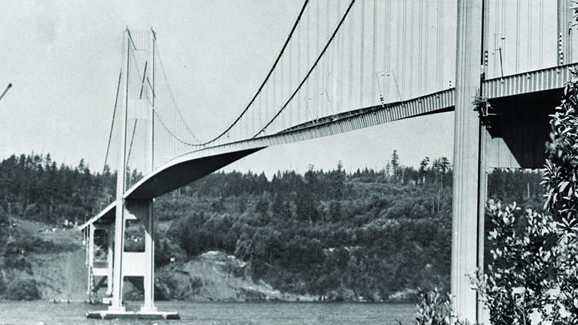
\includegraphics[width=\linewidth]{tac01}
\endminipage\hfill
\minipage{0.33\textwidth}
  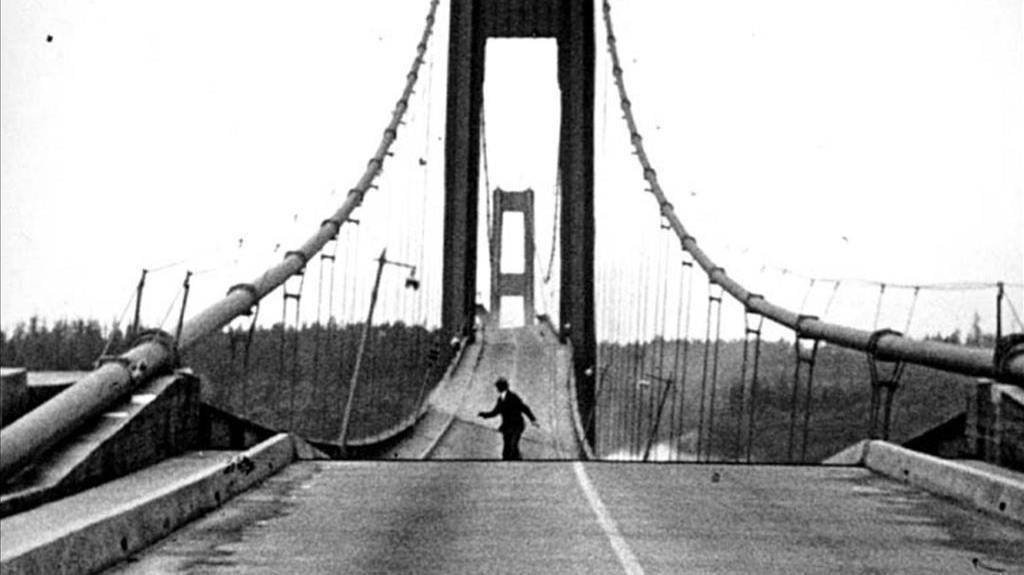
\includegraphics[width=\linewidth]{tac02}
\endminipage\hfill
\minipage{0.33\textwidth}%
  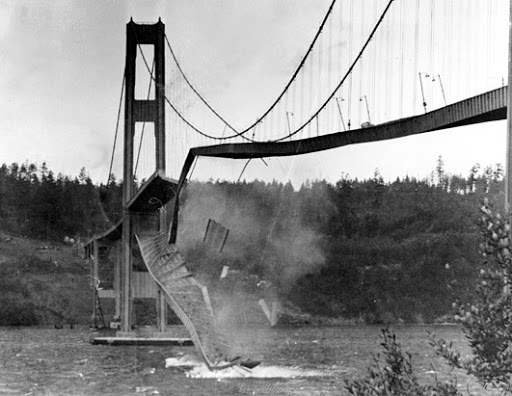
\includegraphics[width=\linewidth]{tac03}
\endminipage
\end{figure}

\noindent{\bf Models:}
Let the vertical deflection
(positive direction downward) of the slice of the roadbed denoted by $y(t)$, where $t$ represents time, and $y=0$ represents the equilibrium position of the road. 

\begin{enumerate}
\item
Here are three simplified second order differential equations that model the situations of the Tacoma Bridge. Assume that at the initial time, the displacement of the bridge $y(0)=0$, and the velocity of the bridge $y'(0)=0.1$,  so that the roadbed
starts in the equilibrium position with a small downward velocity. For each of the following equations, find the solution to the IVP with these initial conditions. Graph the solutions, and describe the short-term and long-term behavior of the solutions.
\begin{enumerate}
\item {\bf Without force.} $\dfrac{d^2y}{dt^2} + 4y = 0$.
\item {\bf With periodic forcing.} $\dfrac{d^2y}{dt^2} + 4y = \cos(t)$.
\item {\bf In resonance.} $\dfrac{d^2y}{dt^2} + 4y = \cos(2t)$.
\end{enumerate}
\begin{framed}
(a) To solve an IVP, we find the general solution, then use the initial conditions.
This is a homogeneous linear ODE with constant coefficients. The auxiliary polynomial is
\[ r^2 + 4 = 0\]
with roots $r=\pm 2i$, so the general solution is
\[ y = C_1 \cos(2t) + C_2 \sin(2t).\]
We plug in the initial conditions:
\[ 0 = y(0) = C_1 \cos(2t) + C_2 \sin(2t) = C_1\]
\[ .1 = y'(0) = -2 C_1 \sin(2t) + 2 C_2 \cos(2t) = 2 C_2 \rsa C_2 = .05\]
\[ y = .05 \sin(2t).\]

This oscillates with the same frequency and same amplitude forever.

(b) To solve this IVP, again we find the general solution, then use the initial conditions. This a a nonhomogeneous linear ODE with constant coefficients. First we find the complementary solution, which is just what we did in part (a):
\[ y = C_1 \cos(2t) + C_2 \sin(2t).\]
Make sure you are using the general complementary solution and not the previous IVP solution here. Now we choose a ``trial solution'': for a target of $\cos(t)$, we take a mystery superposition of $\cos(t)$ and $\sin(t)$:
\[ y_p = A \cos(t) +  B \sin(t)\]
and plug in
\[ y_p' = -A \sin(t) + B\cos(t), \ y''_p = -A \cos(t) - B \sin(t)\]
\[ \rsa (-A \cos(t) - B \sin(t)) + 4 ( A \cos(t) +  B \sin(t)) = \cos(t)\]
\[ \rsa 3A \cos(t) + 3B\sin(t) = \cos(t)\]
\[\rsa A= \frac{1}{3}, \ B= 0\]
\[ y_p  = \frac{1}{3} \cos(t).\]
The general solution is then
\[ y = \frac{1}{3} \cos(t) + C_1 \cos(2t) + C_2 \sin(2t).\]
Only now do we use the initial conditions:
\[ 0 = y(0) = \frac{1}{3} + C_1 \rsa C_1 = - \frac{1}{3}\]
\[ .1 = y'(0) = 0 + 0 + 2 C_2 \rsa C_2 = .05\]
\[ y = \frac{1}{3} \cos(t)  - \frac{1}{3} \cos(2t) + .05 \sin(2t).\]

This oscillates with a larger amplitude than last time, but still bounded.

(c) We follow the same outline. The first thing that changes is our trial solution: we cannot take
\[ y_p = A \cos(2t) +  B \sin(2t)\]
as a ``trial solution'' since these are homogeneous solutions! We fix them by multiplying by $t$:
\[ y_p = A t\cos(2t) +  B t\sin(2t).\]
We follow the same process: plug in the trial solution to the equation to find $A$ and $B$. We get
\[ y_p = \frac{1}{4} t \sin(2t)\]
and
\[ y =  \frac{1}{4} t \sin(2t) + C_1 \cos(2t) + C_2 \sin(2t)\]
as the general solution. Then we plug in the initial conditions to solve for $C_1$ and $C_2$ and we get 
\[ y = \frac{1}{4} t \sin(2t) + .05 \sin(2t).\]

This oscillates with larger and larger waves, without bound!
\href{https://www.geogebra.org/m/bzsn4mmd}{Here are the graphs.}

\end{framed}

\item Perfect coincidences are rare in nature: it's very unlikely for the wind frequency to exactly equal the natural frequency of the bridge.
\begin{enumerate}
\item Before solving, what do you expect to happen to the solution of the IVP with same initial conditions and equation $\dfrac{d^2y}{dt^2} + 4y = \cos(1.9 t)$? 
\item Graph the solution to the IVP described in the last part, and describe the short-term and long-term behavior of the solutions.
\item Repeat the last two questions for $\dfrac{d^2y}{dt^2} + 4y = \cos(1.99 t)$.
\item What happens in the limit with the same IVP with $\dfrac{d^2y}{dt^2} + 4y = \cos(\alpha t)$ as $\alpha \to 2$?
\end{enumerate}

\begin{framed}
Summary: In general for $\dfrac{d^2y}{dt^2} + 4y = \cos(\alpha t)$ with the same initial condition, we have solution
\[ y = \frac{1}{4-\alpha^2} \left(\cos(\alpha t) - \cos(2t)\right) + .05 \sin(2t).\]
If $\alpha$ is very close to $2$, the fraction $\frac{1}{4-\alpha^2}$ is large, and, for a while at least, $\alpha t$ is close to $2t$. For small values of $t$, $\alpha t$ is close to $2t$, so $\cos(\alpha t) - \cos(2t)$ is small, but as $t$ gets larger, this can get large again, but then small again, and so on. So, we get waves that get larger for a while, then smaller again, and so on.

\href{https://www.geogebra.org/m/bzsn4mmd}{Here are the graphs again.}
\end{framed}
\end{enumerate}

\Oct{27}

\subsection{Spring and mass systems (\S5.1)}\index{springs}

Given an object on a spring, its motion is determined by Hooke's law\index{Hooke's law}, which says that the force from the spring is proportional to the displacement of the spring from its resting length, but in the opposite direction. Combined with Newton's second law (force $=$ mass $\times$ acceleration), we can get an equation that governs the total force applied by the spring. First we name variables:
$x$ is the displacement of the mass on the spring from resting position, $t$ is time, $m$ is the mass. We also need some constant of propotionality $k$. We can then write an equation:
\[ m x'' = - k x, \qquad (m,k>0) \]
 or
\[ m x'' + k x = 0,  \qquad (m,k>0). \]
This a homogeneous linear ODE with constant coefficients, so we find the roots of the auxiliary polynomial
\[ m r^2 + k = 0, \rsa r = \pm i \sqrt{\frac{k}{m}}.\]
The general solution is then
\[ x = C_1 \cos(\gamma x) + C_2 \sin(\gamma x),\]
for $\gamma= \sqrt{ \frac{k}{m} }$, so these solutions are all periodic functions of fixed wavelength $\frac{2 \pi}{\gamma}$.

However, there is generally some sort of friction or resistance to the system. We add a friction force in the opposite direction to the spring force:
\[ m x'' = - \beta x' - k x, \qquad (m,\beta,k>0)\]
or
\[ m x'' + \beta x' + k x = 0, \qquad (m,\beta,k>0).\]
The $\beta x'$ term gives a damping effect to the system.

The behavior of the system is determined by the roots of the auxiliary polynomial:
\[ m r^2 + \beta r + k  = 0\]
\[\rsa r_1,r_2= \frac{ - \beta \pm \sqrt{\beta^2- 4 m k }}{2 m}\]
The behavior breaks into three cases:

\begin{enumerate}
\item If $\beta^2- 4 m k>0$, then the roots $r_1,r_2$ are real. Since $m,\beta,k>0$, \[\sqrt{\beta^2- 4 m k } < \sqrt{\beta^2}=\beta,\]
\[ -\beta + \sqrt{\beta^2- 4 m k }<0 \ (\text{and also} \  -\beta + \sqrt{\beta^2- 4 m k }<0),\]
so both roots are negative. The general solution is of the form $x = C_1 e^{r_1t} + C_2 e^{r_2 t}$. Then there are no oscillations, and the spring heads to its resting position. A system like this is called \index{overdamped}\emph{overdamped}.

\begin{center}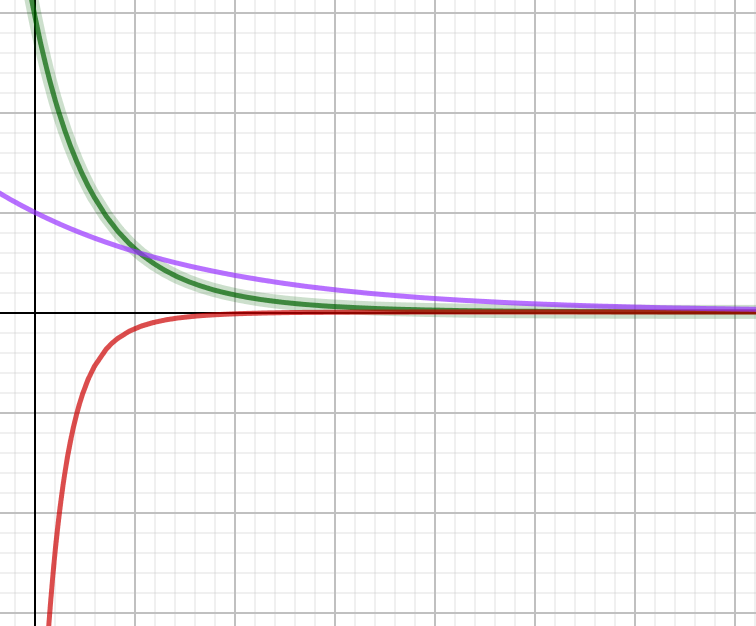
\includegraphics[scale=.5]{spring1}\end{center}

\item If $\beta^2- 4 m k<0$, then the roots $r_1,r_2$ are complex. The real part is $\frac{-\beta}{2m}$, which is negative, and the imaginary part is $\frac{1}{2m}\sqrt{\beta^2- 4 m k } = \frac{1}{2m}\sqrt{-1 (4 m k - \beta^2) } = i \gamma$ for $\gamma=\frac{1}{m}\sqrt{4 m k - \beta^2}$. The general solution is of the form \[x= C_1 e^{-\beta t / 2m } \cos(\gamma t) + C_2 e^{-\beta t / 2m } \sin(\gamma t).\] These solutions oscillate with wavelength $\frac{2\pi}{\gamma}$, and with decreasing amplitude $e^{-\beta t / 2m }$. A system like this is called \index{underdamped}\emph{underdamped}.

\begin{center}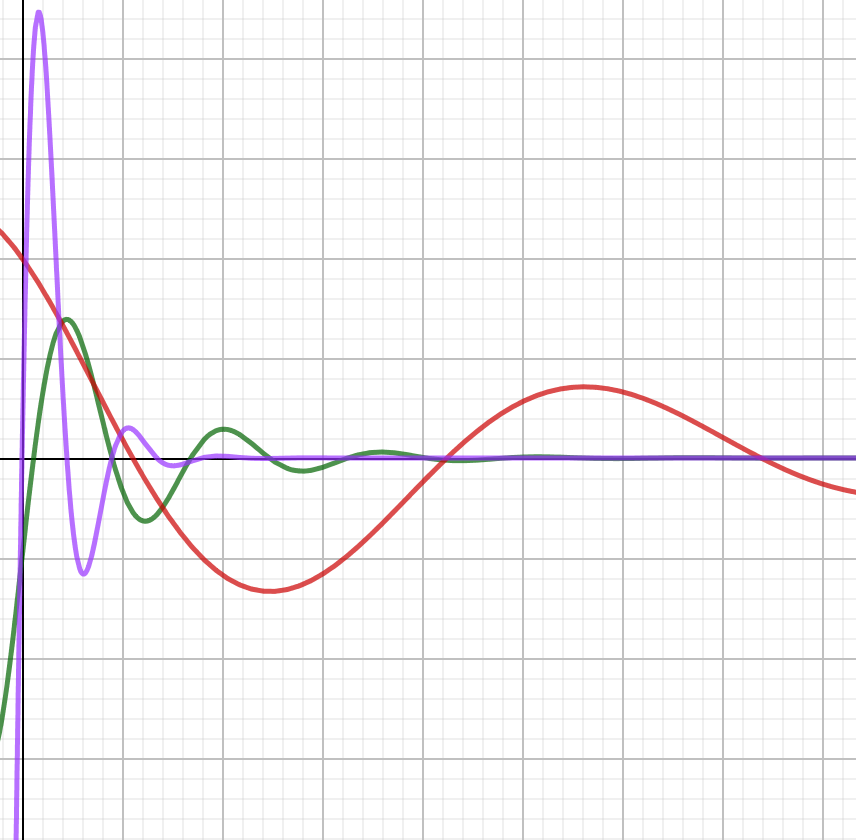
\includegraphics[scale=.5]{spring2}\end{center}


\item If $\beta^2- 4 m k=0$, then there is a repeated real root $r$, which again is negative. The general solution is of the form $x = C_1 e^{r t} + C_2 t e^{r t}$. A system like this is called \index{critically damped}\emph{critically damped}, since a small change will make it overdamped or underdamped.

\begin{center}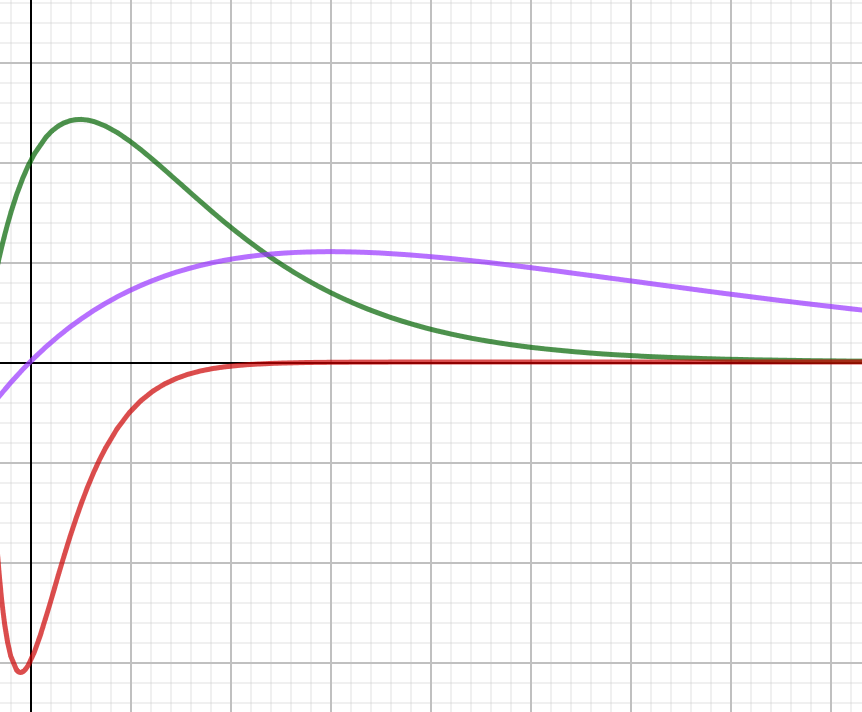
\includegraphics[scale=.5]{spring3}\end{center}
\end{enumerate}


Finally, let's take one example of what can happen if we apply an additional force to our spring system.
\begin{ex}
Consider the initial value problem
\[\begin{cases} x'' + 2 x = \cos(\alpha t)\\
x(0)=0\\
x'(0)=0
\end{cases}\]
for some constant $\alpha$. This corresponds to a mass-spring system with no damping, plus an additional oscillating force with wavelength $\frac{2\pi}{\alpha}$. 
\[ r^2 + 2 = 0 \rsa r = \pm i \sqrt{2},\]
so the homogeneous general solution is
\[ x_c = C_1 \cos(\sqrt{2} t) +  C_2 \sin(\sqrt{2} t).\]
If $\alpha\neq \sqrt{2}$, then the ``trial solution'' is
\[ x_p = A \cos(\alpha t) + B \sin(\alpha t),\] and after subbing and solving, we get the solution to the IVP
\[ x(t) = \frac{1}{2-\alpha^2} \left( \cos(\alpha t) - \cos( \sqrt{2} t) \right).\]
For $\alpha=1,\ 2, \ 1.3$, we have
\begin{center}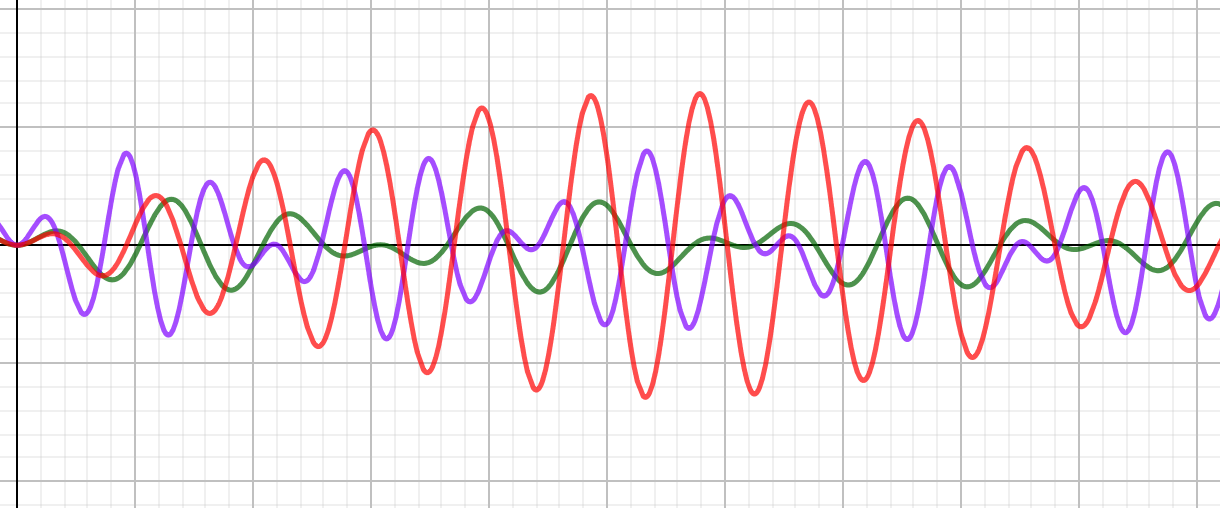
\includegraphics[scale=.5]{spring4}\end{center}
In particular, all of these solutions are bounded, and somewhat repeating.

What about $\alpha=\sqrt{2}$? Then our first guess for the ``trial solution'' is again
\[ x_p = A \cos(\alpha t) + B \sin(\alpha t),\]
but this is part of the complementary solution! We multiply by $t$ to correct it:
\[ x_p = A t \cos(\sqrt{2} t) + B t \sin(\sqrt{2} t),\]
and after subbing and solving, we get the general solution
\[ x= \frac{1}{2\sqrt{2}} t \sin(\sqrt{2} t) + C_1 \cos(\sqrt{2} t) +  C_2 \sin(\sqrt{2} t),\]
and IVP solution
\[ x= \frac{1}{2\sqrt{2}} t \sin(\sqrt{2} t).\]

\begin{center}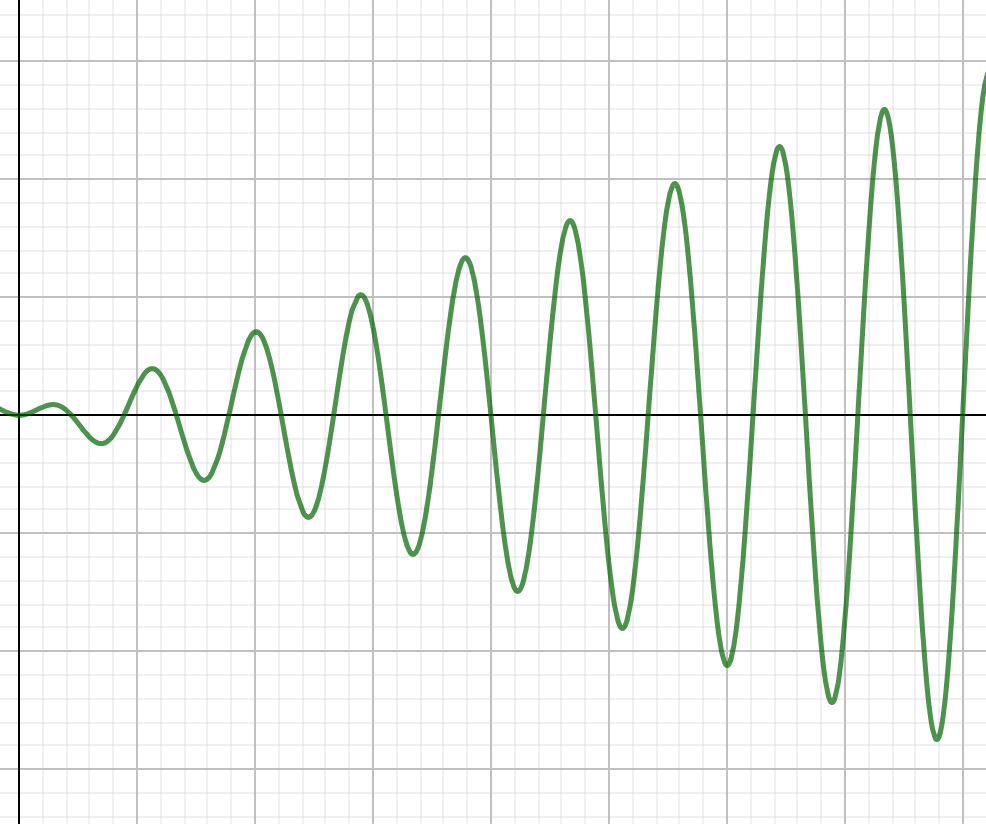
\includegraphics[scale=.5]{spring5}\end{center}

The solution gets larger and larger and larger!
This is an example of \index{resonance}\emph{resonance}.
\end{ex}

\subsection*{Laplace Transforms (\S7.1)}

Our next big topic is a general method to translate differential equations to simpler algebraic equations (which are then easier to solve). Here is the basic idea. To a function $f(t)$, we will associate another function $\LA{f(t)}$ called its \emph{Laplace transform}\index{Laplace transform}, which is a function of another variable $s$. We will think of the Laplace transform of $f$ as another function that is its evil twin\index{evil twin}. We might write something like $F(s) = \LA{f(t)}(s)$ to say that the function $F$ with input variable $s$ is the Laplace transform of the function $f$ whose input variable is $t$; the $\La$ is telling us the function $F$ we are specifying is the Laplace transform of $f$. The upshot is that derivatives in regular world will correspond to multiplication by $s$ in Laplace transform (evil twin) world.



\Nov{1}

\begin{defn} Let $f(t)$ be a function defined for all $t\geq 0$. The \emph{Laplace transform}\index{Laplace transform} is the function $\LA{f(t)}$ is the function of $s$ given by the rule
\[ \LA{f(t)}(s) = \int_0^\infty e^{-st} f(t) \, dt,\]
provided this interval converges.
\end{defn}

This is a function of $s$, because for every different value of $s$ we choose, we get a different integral from $0$ to $\infty$, which is a number (as long as it converges). Sometimes we'll write $F(s)$ as shorthand for $ \LA{f(t)}(s)$ just to make it easier to work with.


\begin{ex} Let's compute $\LA{1}$ from the definition:
\[ \LA{1}(s) = \int_0^\infty e^{-st} \cdot 1 \, dt = \left[ \frac{-1}{s} e^{-st} \right]_{0}^{\infty} = \lim_{t\to\infty}\frac{-1}{s} e^{-st} - \left(\frac{-1}{s}\right)\]
For $s>0$, the limit $\lim_{t\to\infty}\frac{-1}{s} e^{-st}$ is zero, while for $s \leq 0$, the limit $\lim_{t\to\infty}\frac{-1}{s} e^{-st}$ does not exist. We conclude that
\[ \LA{1}(s) = \frac{1}{s}\]
on the domain $s>0$.
\end{ex}

\begin{ex} Let's compute $\LA{e^{5t}}$ from the definition, for some real number $r\neq 0$:
\begin{align*} \LA{e^{5t}}(s) = \int_0^\infty e^{-st} &\cdot e^{5t} \, dt = \int_0^\infty e^{(5-s)t} \, dt = \left[ \frac{1}{5-s} e^{(5-s)t} \right]_{0}^{\infty} \\&= \lim_{t\to\infty}\frac{1}{5-s} e^{(5-s)t} - \left(\frac{1}{5-s}\right) = \frac{-1}{5-s} = \frac{1}{s-5},\end{align*}
for $s>5$.

By basically the same computation, $\LA{e^{at}} = \frac{1}{s-a}$ for any real number $a\neq 0$ on the domain $s>a$.
\end{ex}

\renewcommand{\arraystretch}{2.5}

With slightly more annoying integration, we can obtain the following table:
\begin{center}
\begin{tabular}{|c|c|}
 \hline
function $f(t)$ & Laplace $\LA{f(t)}(s)$\\
  \hline
$1$ &$ \displaystyle\frac{1}{s} \quad \ (s>0)$
 \\  \hline
 $t^n$ & $ \displaystyle\frac{n!}{s^{n+1}} \quad \ (s>0)$
 \\  \hline
  $e^{at}$ & $ \displaystyle\frac{1}{s-a} \quad (s>a)$
 \\  \hline
  $\sin(kt)$ & $ \displaystyle\frac{k}{s^2 + k^2} \quad (s>0)$
 \\  \hline
   $\cos(kt)$ & $ \displaystyle\frac{s}{s^2 + k^2} \quad (s>0)$
 \\  \hline
%   $\sinh(kt)$ & $ \displaystyle\frac{k}{s^2 - k^2} \quad (s>k)$
% \\  \hline
%   $\cosh(kt)$ & $ \displaystyle\frac{s}{s^2 - k^2} \quad (s>k)$
% \\  \hline
\end{tabular}
\end{center}

\

We will take these as the building blocks. We can also take Laplace transforms of superpositions of functions whose Laplace transforms we already know: 
If $f_1(t)$ and $f_2(t)$ are functions whose Laplace transforms we know, and $c_1, c_2$ are constants, then
\begin{align*} \LA{c_1 f_1(t) &+ c_2 f_2(t)}(s) = \int_0^\infty e^{-st} (c_1 f_1(t) + c_2 f_2(t))\, dt \\&= \int_0^\infty c_1 e^{-st}  f_1(t) + c_2 e^{-st}f_2(t))\, dt \\&= 
c_1 \int_0^\infty  e^{-st}  f_1(t) \, dt + c_2  \int_0^\infty  e^{-st}f_2(t))\, dt \\&= c_1 \LA{f_1(t)}(s) + c_2 \LA{f_2(t)} (s)\end{align*}

That is, Laplace transforms satisfy the same ``sum rule'' and ``constant rule'' that integrals satisfy.



\subsection*{Discussion Questions}

\begin{enumerate}
\item Find the Laplace Transforms $F(s)$ of the following functions:
\begin{enumerate}
\item $f(t)=3 e^{7t}$.
\item $f(t)=-4 t^2 + 7t$.
\item $f(t)=\sqrt{2} \cos(3 t) + \sqrt{5} \sin(7t)$.
\end{enumerate}
\item Find functions $f(t)$ whose Laplace Transforms are the following functions:
\begin{enumerate}
\item $F(s) = \displaystyle \frac{2}{s^3}$.
\item $F(s) = \displaystyle \frac{8}{s^3}$.
\item $F(s) = \displaystyle \frac{2}{s-3} - \frac{7}{s+1}$.
%\item $F(s) = \displaystyle \frac{2s+4}{s^2 + 9}$.
\end{enumerate}
\end{enumerate}
\begin{framed}
\begin{enumerate}
\item \begin{enumerate}
\item $F(s) = \displaystyle \frac{3}{s-7}$.
\item $F(s) = \displaystyle -4 \frac{2!}{s^3} +7 \frac{1!}{s^2} = \frac{7s-8}{s^3} $.
\item $F(s) = \displaystyle \sqrt{2}\frac{s}{s^2+9} + \sqrt{5} \frac{7}{s^2 + 49}$.
\end{enumerate}
\item \begin{enumerate}
\item $f(t) = t^2$.
\item $f(t) = 4t^2$.
\item $f(t) = 2e^{3t} - 7 e^{-t}$.
%\item $F(s) = \displaystyle \frac{2s+4}{s^2 + 9}$
\end{enumerate}
\end{enumerate}
\end{framed}

\begin{defn}
The \emph{inverse Laplace transform}\index{inverse Laplace transform} of a function $F(s)$ is the function $f(t)$ whose Laplace transform is $F(s)$. We write $\LAi{F(s)}$ for the inverse Laplace transform of $F(s)$.
\end{defn}

Thus, $f(t) = \LAi{F(s)}$ $\Leftrightarrow$ $F(s) = \LA{f(t)}$.

To compute inverse Laplace transforms, we can read our table of Laplace transforms from right to left and use the fact that the inverse Laplace transform behaves well with superpositions.



\Nov{3}

%\begin{ex}
%\[\begin{aligned} \LAi{\frac{2s+7}{s^2+16}} &= 2 \LAi{\frac{s}{s^2+16}} + 7 \LAi{\frac{1}{s^2+16}} \\&= 2 \LAi{\frac{s}{s^2+16}} + \frac{7}{4} \LAi{\frac{4}{s^2+16}} = 2 \cos(4t) + \frac{7}{4}\sin(4t).\end{aligned}\]
%\end{ex}


It is not clear that these indefinite integrals should always converge. They don't always!
\begin{ex}
The function $f(t)= e^{t^2}$ does not have a Laplace transform:
\[ \LA{e^{t^2}}(s) =  \int_0^\infty e^{-st} \cdot e^{t^2} \, dt = \int_0^s e^{t^2-st}  \, dt + \int_s^\infty e^{t^2-st}  \, dt,\]
which diverges since for $t\geq s$ , $t^2-st\geq 0$ and hence $e^{t^2-st}\geq 1$.
\end{ex}

 However:
\begin{fact}
Given a piecewise continuous function $f(t)$, if there is some exponential function $e^{at}$ such that $f(t)\leq e^{at}$ for all sufficiently large values of $t$, then $f$ has a Laplace transform, meaning that the integrals involved in computing the Laplace transforms converge for all sufficiently large $s$.
\end{fact}



Now we discuss the main point behind Laplace transforms. Let's take a function $f(t)$ and its derivative $f'(t)$ and compute the Laplace transform of the derivative. By the definition:

\[ \LA{f'(t)} = \int_{0}^\infty f'(t) e^{-st} \ dt\]
To compute this, we apply integration by parts: 
\[u=e^{-st}, \ du = -s e^{-st} \, dt,  \ dv = f'(t) \, dt,  \ v=f(t)\]
\[ \rsa \int_{0}^\infty f'(t) e^{-st} \ dt = \left[ f(t) e^{-st} \right]_{t=0}^\infty - (-s) \int_{0}^\infty f(t) e^{-st} \ dt\]
\[ \rsa \LA{f'(t)}(s) = (0 - f(0))  + s \LA{f(t)}(s) = s \LA{f(t)}(s) - f(0).\]
In shorthand if we put $F(s)$ for $\LA{f(t)}(s)$, this reads
\[  \LA{f'(t)}(s) = s F(s) - f(0).\]
What's the point of this calculation? Derivatives in the regular world translate into multiplication by $s$ in Laplace transformation world!

If we repeat this calculation, we get
\begin{align*}
\LA{f''(t)}(s) &= s \LA{f'(t)}(s) - f'(0)\\&= s( \LA{f(t)}(s) - f(0) ) - f'(0)\\
&= s^2 \LA{f(t)}(s) - s f(0) - f'(0)
\end{align*}
and in general
\[ \LA{f^{(n)}(t)}(s) = s^n \LA{f(t)}(s) - s^{n-1} f(0) - s^{n-2} f'(0) - \cdots - f^{(n-1)}(0).\]

We can use Laplace transforms to transform initial value problems into algebraic equations.

\begin{ex} Consider the IVP
\[ \begin{cases} y' - 2y = 0 \\ y(0) = 5\end{cases}.\]
Let's apply Laplace transforms to both sides:
\[ \LA{ y' - 2y} = \LA{0}\]
\[\rsa \LA{y'} - 2 \LA{y} = 0\]
For convenience we will use $Y$($=Y(s)$) for $\LA{y}$.
\[ \rsa (sY - y(0)) - 2 Y =0\]
\[ \rsa (sY - 5) - 2 Y =0\]
\[ \rsa (s-2)Y = 5\]
\[ \rsa Y = \frac{5}{s-2}\]
Then we translate back to actual functions with the inverse Laplace transform:
\[ \rsa y = \LAi{\frac{5}{s-2}} = 5 \LAi{\frac{1}{s-2}} = 5 e^{2t}.\]
\end{ex}

We will often get fraction equations when applying this method, so we might need to apply partial fractions.

\subsection*{Quick review of partial fractions}
Given a rational function $\frac{p(x)}{q(x)}$ with $\deg(p)<\deg(q)$, we can often use partial fractions\index{partial fractions} to write this as a sum of fractions with simpler denominators.

\begin{itemize}
\item When $q(x) = L_1 L_2$ has two distinct linear factors, we write
\[ \frac{p(x)}{q(x)} = \frac{A}{L_1} + \frac{B}{L_2}.\]
Then clear denominators and solve for $A$ and $B$:
\[ p(x) = A L_2 + B L_1.\]
We can either just make a constant coefficient equation and an $x$-coefficient equation and solve that system for $A$ and $B$, or we can be more clever and plug in $x=$ root of $L_1$ and $x=$ root of $L_2$ to get simple equations.

For example,
\[ \frac{5x+4}{x(x-2)} = \frac{A}{x} + \frac{B}{x-2}\]
\[\rsa 5x+4 = A(x-2) + Bx.\]
Let's be clever: plug in $x=0$
\[ \rsa 4 = 5\cdot 0 + 4 = A (0-2) + B \cdot 0 = -2A \rsa A=-2\]
and $x=2$
\[ \rsa 14 = 5 \cdot 2  + 4 = A (2-2) + B \cdot 2 = 2B \rsa B=7\]
so
\[ \frac{5x+4}{x(x-2)} = \frac{-2}{x} + \frac{7}{x-2}.\]

\item When $q(x) = L_1 Q_1$ has a linear and an irreducible quadratic factor, we write
\[ \frac{p(x)}{q(x)} = \frac{A}{L_1} + \frac{Bx+C}{Q_1}.\]
Then clear denominators and solve for $A,B,$ and $C$:
\[ p(x) = A Q_1 + (Bx+C) L_1.\]
We can either just make a system of equations for the $1,x,x^2$-coefficients, or we can be more clever and plug in $x=$ root of $L_1$ to get started.

For example,
\[ \frac{1}{(x-1)(x^2+9)}= \frac{A}{x-1} + \frac{Bx+C}{x^2+9}\]
\[ \rsa 1= A(x^2+9) + (Bx+C)(x-1).\]
To be clever, plug in $x=1$ to get
\[ 1 = A(1^2+9) + (B \cdots 1 + C) (1-1) = 10 A \rsa A=\frac{1}{10}.\]
Then 
\[1= \frac{1}{10}(x^2+9) + (Bx+C)(x-1) = (\frac{1}{10} + B) x^2 + (C-B) x + (\frac{9}{10} - C)\]
so $C-B=0$ so $B=C$, and $B+\frac{1}{10} = 0$, so $B=C=-\frac{1}{10}$. Thus,
\[\frac{1}{(x-1)(x^2+9)}= \frac{\frac{1}{10}}{x-1} - \frac{\frac{1}{10}x+\frac{1}{10}}{x^2+9}.\]

\item When $q(x)=L_1^2$ has a double linear factor,  we write
\[ \frac{p(x)}{q(x)} = \frac{A}{L_1} + \frac{B}{L_1^2}.\]
Again clear denominators to get
\[ p(x) = A L_1 + B\]
and solve for $A,B$. You can plug in the root of $L_1$ for $x$ to get  $B$ if you want to be clever.
\end{itemize}

\subsection*{Solving IVPs with Laplace transforms}

\begin{ex}
Consider the IVP
\[ \begin{cases} y' - 2y = 4 \\ y(0) = 5\end{cases}.\]
Let's apply Laplace transforms to both sides:
\[ \LA{ y' - 2y} = \LA{4}\]
\[\rsa \LA{y'} - 2 \LA{y} = \frac{4}{s}\]
For convenience we will again use $Y$($=Y(s)$) for $\LA{y}$.
\[ \rsa (sY - y(0)) - 2 Y =\frac{4}{s}\]
\[ \rsa (sY - 5) - 2 Y =\frac{4}{s}\]
\[ \rsa (s-2)Y = 5+\frac{4}{s} = \frac{5s+4}{s}\]
\[ \rsa Y = \frac{5s+4}{s(s-2)}.\]

To prepare for computing the inverse Laplace transform, we use partial fractions. We did this example above!
\[ \frac{5s+4}{s(s-2)} = \frac{-2}{s} + \frac{7}{s-2}.\]
Then we translate back to actual functions with the inverse Laplace transform:
\[ \rsa y = \LAi{\frac{-2}{s} + \frac{7}{s-2}} = -2 \LAi{\frac{1}{s}} + 7 \LAi{\frac{1}{s-2}} = -2 + 7e^{2t}.\]
\end{ex}

\begin{ex}
Consider the IVP
\[ \begin{cases} y'' +9y = e^t \\ y(0) = 0 \\ y'(0)=0\end{cases}.\]
Let's apply Laplace transforms to both sides:
\[ \LA{  y'' +9y = e^t} = \LA{e^t}\]
\[\rsa \LA{y''} + 9 \LA{y} = \frac{1}{s-1}\]
For convenience we will again use $Y$($=Y(s)$) for $\LA{y}$.
\[ \rsa (s^2Y - sy(0)-y'(0)) +9 Y =\frac{1}{s-1}\]
\[ \rsa (s^2+9)Y=\frac{1}{s-1}\]
\[ \rsa Y =\frac{1}{(s-1)(s^2+9)}\]

To prepare for computing the inverse Laplace transform, we use partial fractions. We did this example above!
\[ \frac{1}{(s-1)(s^2+9)} = \frac{\frac{1}{10}}{s-1} - \frac{\frac{1}{10}x+\frac{1}{10}}{s^2+9}. \]
Then we translate back to actual functions with the inverse Laplace transform:
\begin{align*} y &= \LAi{\frac{\frac{1}{10}}{s-1} - \frac{\frac{1}{10}s+\frac{1}{10}}{s^2+9}} \\&=\frac{1}{10} \LAi{\frac{1}{s-1}} - \frac{1}{10} \LAi{\frac{s}{s^2+9}}  - \frac{1}{30} \LAi{\frac{3}{s^2+9}} \\&= \frac{1}{10} e^t- \frac{1}{10} \cos(3t)-\frac{1}{30} \sin(3t).
\end{align*}
\end{ex}

\begin{comment}

\Nov{15}



\subsection*{Translation theorems for Laplace transforms (\S7.3)}

Recall that if $g(x)$ is a function, then $g(x-a)$ is the function you get by shifting the graph to the right by $a$ (if $a$ is positive; to the left by $|a|$ if $a$ is negative); we sometimes call this function a \emph{translation}\index{translation} of $g$. Following the webwork, we might use notation like $g|_{x-a}$\index{$g|_{x-a}$} for this sometimes.

Translating a Laplace transform has a nice formula:

\begin{thm} If $\LA{f(t)} = F(s)$ then
\[ \LA{e^{at} f(t)} = F(s-a).\]
\end{thm}

We can also write this as $\LA{e^{at} f(t)} = F|_{s-a}$.
This is easy to check:
\[ \LA{e^{at} f(t)}(s) = \int_{0}^\infty e^{-st} e^{at} f(t) \ dt = \int_{0}^\infty e^{-(s-a)t} f(t) \ dt = F(s-a).\]

For a simple example, the theorem says that 
\[\LA{ e^{5t} \sin(6x)} = \LA{\sin(6x)}|_{s-5} = \frac{6}{(s-5)^2 + 36}.\]

The theorem is especially useful in computing inverse Laplace transforms. We can rewrite the formula above as:
\[ \LAi{F|_{s-a}} = e^{at} \LAi{F}.\]

\begin{ex} To compute the inverse Laplace transform of $F(s) = \frac{5}{(s+3)^2}$, first we realize this function as $\frac{5}{s^3}|_{s+2}$. Then 
\[\LAi{F(s)} = \LAi{\frac{5}{s^3}|_{s+2}}  = e^{-2t} \LAi{\frac{5}{s^3}} = \frac{5}{2} e^{-2t} \LAi{\frac{2}{s^3}} =\frac{5}{2} t^2.\]
\end{ex}

We can also compute inverse Laplace transforms of irreducible quadratics use this theorem and completing the square. Recall that \emph{completing the square}\index{completing the square} is an algebraic technique to rewrite quadratic polynomials: to rewrite $x^2 + bx + c$, we split $b$ in half and write
\[ x^2 + bx + c = (x+\frac{b}{2})^2 + d\]
and solve for $d$.
For example,
\[ x^2 + 4x + 7 = (x+2)^2 + d = (x^2 + 4x + 4) + d \rsa d=3\]
\[ \rsa x^2 + 4x + 7 = (x+2)^2 + 3.\]

\begin{ex}
Let's compute the inverse Laplace transform of
\[ F(s) = \frac{sx - 7} {s^2 + 6s + 13}.\]
First we apply completing the square to the bottom:
\[ s^2 + 6s + 13 = (s+3)^2 + d = s^2 + 6s + 9 + d \rsa d=4\]
\[ \rsa s^2 + 6s + 10 = (s+3)^2 + 4,\]
so 
\[ F(s) = \frac{2s - 7} {(s+3)^2 + 4}.\]
Now, we would like to think of $(s+3)^2 + 4$ as a function of $s+3$. We rewrite the numerator accordingly:
\[ 2s-7 = 2(s-3 + 3) - 7 = 2(s-3) + 6 - 7 = 2(s-3)-1,\]
so
\[ F(s) =  \frac{2(s-3)-1} {(s+3)^2 + 1} = \frac{2s-1}{s^2+4} |_{s+3}.\]
Thus, by the theorem,
\[ \LAi{F(s)} = e^{-3t} \LAi{\frac{2s-1}{s^2+4}} =e^{-3t}\left( 2\LAi{\frac{s}{s^2+4}} - 1\LAi{\frac{1}{s^2+4}}\right) \] 
\[ = e^{-3t}\left( 2\LAi{\frac{s}{s^2+4}} - \frac{1}{2}\LAi{\frac{2}{s^2+4}}\right) =e^{-3t} (2 \cos(2t) - \frac{1}{2} \sin(2t))\]
\[ = 2 e^{-3t} \cos(2t) - \frac{1}{2}e^{-3t} \sin(2t).\]
\end{ex}

\subsection*{Heaviside functions and second translation theorem}

We will get a very useful rule that allows us to work easily with piecewise defined functions. We start with a building block.

\begin{defn} The \emph{Heaviside function}\index{Heaviside function} or \emph{unit step function}\index{unit step function} is the function
\[ \U(t) = \begin{cases} 1 &\text{if} \ x\geq 0 \\ 0 &\text{if} \ x < 0 \end{cases}.\]
\end{defn}

This is like an on/off switch that turns on at $t=0$. We can translate it to make on/off switches at different times:

The function $\U(t-a)$ is given by the rule
\[ \U(t) = \begin{cases} 1 &\text{if} \ x\geq a \\ 0 &\text{if} \ x < a \end{cases}.\]

If we want to ``switch on'' at $t=a$ and ``switch off'' later at $t=b$, we want the function
\[ \begin{cases} 0 &\text{if} \ x < a \\ 
1 &\text{if} \ a \leq x < b \\
0 &\text{if} \ x>b \end{cases},\]
which is given by
\[ \U(t-a) - \U(t-b).\]

Let's use Heaviside functions to write the function
\[ f(t) = \begin{cases} 2 \cos(4t) &\text{if} \ x \geq 6\pi \\
0 &\text{if} \ x < 6\pi \end{cases}.\]
We want a $2 \cos(4t)$ to be ``on'' starting from $6\pi$, so we take
\[ f(t) = 2 \cos(4t)\, \U(t-6\pi).\]
What about 
\[ g(t) = \begin{cases} 2 \cos(4t) &\text{if} \ 6 \pi \leq x < 8\pi \\
0 &\text{otherwise} \end{cases}?\]
We want a $2 \cos(4t)$ times an on/off switch that's on from $6 \pi$ to  $8\pi$:
\[ g(t) = 2 \cos(4t) ( \U(t-6 \pi) - \U(t-8 \pi) ).\]

Here's how we deal with the Laplace transforms of these:

\begin{thm} If $\LA{f(t)} = F(s)$ then
\[ \LA{f(t-a)\, \U(t-a)} = e^{-as} F(s).\]
\end{thm}

We can write this backwards as 
\[ \LAi{e^{-as} F(s)} = f(t-a)\, \U(t-a) =\LAi{F(s)}|_{t-a}\, \U(t-a).\]

\begin{ex} Let's compute $\LA{ 2 e^{3t} \U(t-5)}$.
We need to rewrite in terms of $t-5$ to use the formula:
\[ \LA{ 2 e^{3t}\, \U(t-5)} = \LA{ 2 e^{3(t-5 + 5)}\, \U(t-5)= \LA{ 2 e^{15} e^{3(t-5)}\, \U(t-5)}} \]
\[= 2 e^{15} e^{-5s} \LA{e^{3t}} = 2 e^{15} \frac{e^{-5s}}{s-5}\]
\end{ex}

\begin{ex} Let's compute $\displaystyle\LAi{ \frac{s}{s^2+9} e^{-\pi s}}$.
We have
\[ \LAi{ \frac{s}{s^2+9} e^{-\pi s}} = \cos(3t)|_{t-\pi}\, \U(t-\pi) \] \[= \cos(3(t-\pi)) \U(t-\pi) = \cos(3t-3\pi) \U(t-\pi).\]
\end{ex}

\subsection*{Discussion Questions}

\begin{enumerate}
\item Find Laplace transforms of the following functions:
\begin{itemize}
\item $f(t)= e^{-2t} \sin(3t)$
\item $g(t) = \begin{cases} 0 &\text{if} \ t< \pi\\
\sin(2t) & \text{if} \ t\geq \pi\end{cases}.$
\item $h(t) = \begin{cases} \sin(2t) & \text{if} \ \pi \leq t < 2\pi \\ 0 & \text{otherwise}\end{cases}$.
\end{itemize}
\begin{framed}
\begin{itemize}
\item $\displaystyle F(s) = \frac{3}{(s+2)^2 +9}$
\item $\displaystyle G(s) = e^{-\pi s} \frac{2}{s^2+4}$.
\item $\displaystyle H(s)= (e^{-\pi s} - e^{-2\pi s}) \frac{2}{s^2+4}$.
\end{itemize}
\end{framed}

\item Find inverse Laplace transforms of the following functions:
\begin{itemize}
\item $\displaystyle F(s) = \frac{6}{s^2 + 8s + 25}$.
\item  $\displaystyle G(s)= \frac{e^{-2s}}{s-4}$.
\end{itemize}

\begin{framed}
\begin{itemize}
\item $\displaystyle f(t)=2 e^{-4t} \sin(3t)$
\item$\displaystyle g(t)= \begin{cases} e^{4t-8} &\text{if} \ t\geq 2 \\ 0 &\text{if} \ t<2\end{cases}$.
\end{itemize}
\end{framed}


\item Use Laplace transforms to solve the following initial value problems:
\begin{itemize}
\item $\begin{cases} y'' + 2y' + 10y = 5\\ y(0)= 0\\ y'(0)=0\end{cases}$.
\item $\begin{cases} y' + y = \begin{cases}  0 &\text{if} \ t< \pi\\
\sin(2t) & \text{if} \ t\geq \pi \end{cases} \\ y(0)= 0\end{cases}$.
\end{itemize}
\end{enumerate}

\begin{framed}
\begin{itemize}
\item $y= \frac{1}{2} + \frac{-1}{2}e^{-t} \cos(3t) - \frac{1}{6} e^{-t} \sin(3t)$.
\item
\end{itemize}
\end{framed}

\subsection*{Dirac delta function (\S7.5)}

Suppose we consider the same amount of total force applied over smaller and smaller time intervals. One way to model this is by a sequence of functions

\[ \delta_a(t) = \begin{cases} \frac{1}{2a} &\text{if} \ -a \leq t \leq a \\ 0 &\text{otherwise}\end{cases}.\]

If we wanted to model a total force of $1$ instantaneously, this would correspond to taking the limit as $a\to 0$. The result is not a function, but it is similar enough to one that we work with it like one anyway. We set
\[ \delta(t) ``= \lim_{a\to 0} \delta_a(t)"\]
and call it the \emph{Dirac delta function}\index{Dirac delta function}. We treat this like a ``function'' that is zero except at $t=0$, and its integral over any interval containing zero is $1$. It is an instantaneous spike that has some area (=1) under the curve.

We can likewise shift and get
\[ \delta(t-a)\]
a delta function centered at $t=a$.

\begin{theorem} 
For $a>0$,
\[ \LA{\delta(t-a)} = e^{-sa}.\]
\end{theorem}

\begin{ex} Consider the initial value problem
\[ \begin{cases} y'' + y = 2\delta(t-2\pi)\\
y(0)=0\\
y'(0)=0\end{cases}.\]
The $y'' + y$ part of the equation is the sort of thing arising from a mass-spring system with no friction. The $2 \delta(t-\2pi)$ on the right hand side corresponds to an instantaneous force at time $2\pi$. Let's solve the IVP with Laplace transforms.
Transforming both sides gives
\[ (s^2+1) Y = 2 e^{-2\pi s},\]
so $Y= \frac{2}{s^2+1}e^{-2\pi s}$.
Then transforming back gives\dots.
\end{ex}

\begin{comment}
\end{comment}

\printindex

\end{document}













 